\documentclass{beamer}
\usepackage[italian]{babel}
\usepackage[T1]{fontenc}
\usepackage[lighttt]{lmodern}
\usepackage{verbatim, listings}

\newcommand{\tile}{TILE\textit{Pro}64}
\newcommand{\musec}{$\mu \textrm{sec}$}
\newcommand{\Lcom}{\mathrm{L}_{\mathrm{com}}}
\newcommand{\Tc}{\mathrm{T}_{\mathrm{C}}}
%% \institute{Laurea Triennale in Informatica}
%% \subtitle{blabla bla}
%% \logo{
\includegraphics[width=15mm]{cherubino_black.pdf}}

\title{Supporto a Meccanismi di Comunicazione per Architetture Many-Core}
\author[Federico Mariti]{{\small Candidato:}\hspace{18ex}  {\small Relatore:} \\ \hspace{3ex}Federico Mariti \hspace{8ex} prof. Marco Vanneschi}
\date{21 giugno 2013}

\begin{document}

\maketitle

\section{Il lavoro svolto: obiettivi e motivazioni}

\begin{frame}
  \frametitle{Il lavoro svolto: obiettivi e motivazioni}
  \begin{itemize}
  \item Prime sperimentazioni sull'uso di Network on Chip per la realizzazione di un supporto ottimizzato alle comunicazioni tra processi.
  \item Nuovo approccio all'implementazione del supporto.
  \item Lo studio \`e realizzato sul Chip~MultiProcessor Tilera~\tile.
  \item Sono realizzate due implementazioni del supporto:
    \begin{itemize}
      \item una che utilizza la memoria condivisa;
      \item l'altra che usa la rete di interconnessione messa a disposizione dal processore.
    \end{itemize}
  \end{itemize}
\end{frame}

\begin{frame}
  \frametitle{Reti di interconnessione del Tilera \tile}
  \begin{figure}
    \resizebox{\columnwidth}{!}{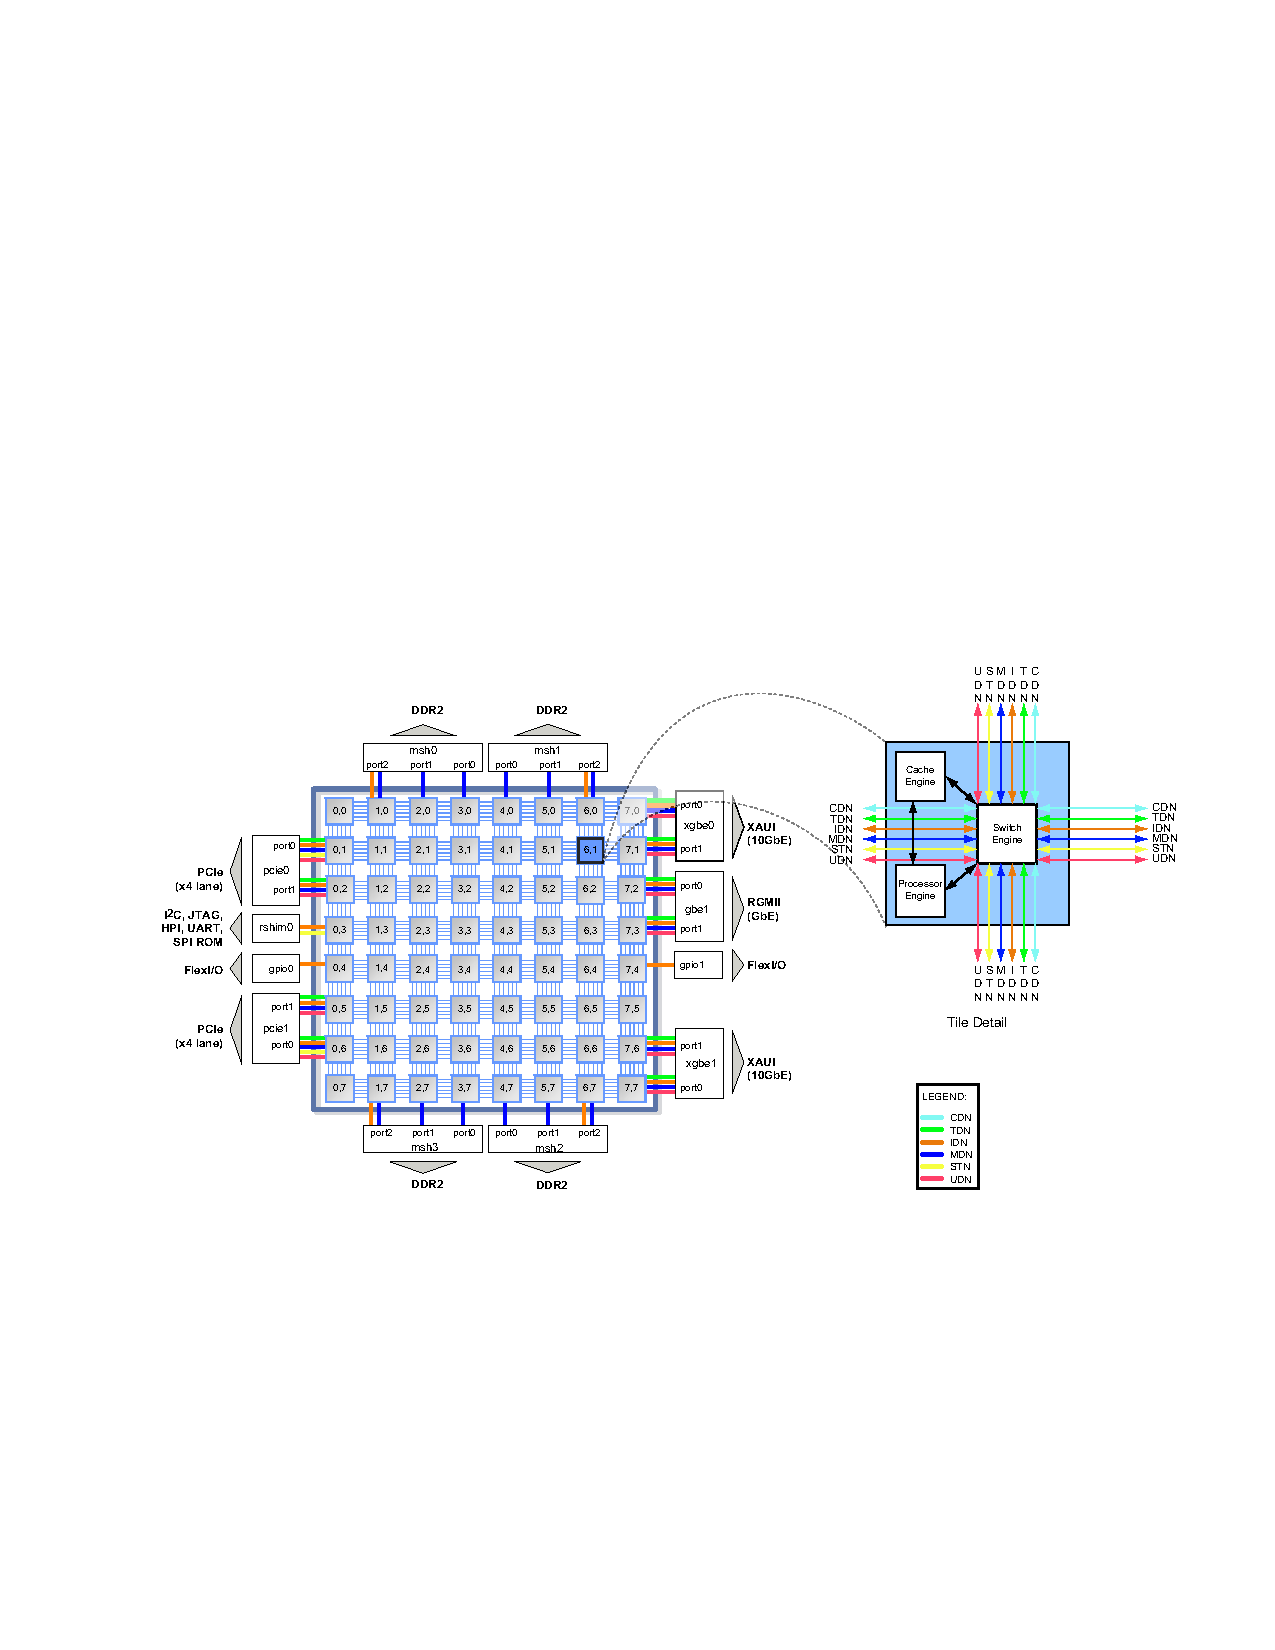
\includegraphics{TilePro64_schema.pdf}}
  \end{figure}
\end{frame}

\begin{frame}
  \frametitle{Dominio Applicativo}
   Computazioni con calcolo di grana fine:
    \begin{description}
    \item [Data Stream Processing] uno o pi\`u flussi contigui, rapidi e varianti nel tempo di dati; l'elaborazione sui dati in ingresso \`e fatta on-line:\hfill
      \begin{itemize}
      \item Monitoraggio e sicurezza di reti informatiche;
      \item Applicazioni finanziarie;
      \item Monitoraggio di sensori e Gestione delle emergenze;
      \item Altri \ldots
      \end{itemize}
    \item [Data Parallel] forma di parallelismo applicabile sia a computazioni su stream che su dato singolo; \`e caratterizzata dal partizionamento dei dati.
      \begin{itemize}
      \item anche su dato singolo, in particolare per la realizzazione delle comunicazioni collettive e nelle forme \emph{Stencil}
      \end{itemize}
    \end{description}
\end{frame}

\note{A scopo esemplificativo si considera una parte di una applicazione su stream riguardante due moduli collegati in pipeline: si assume che il tempo di calcolo del primo modulo sia opportunamente dimensionato come il tempo di interarrivo dello stream. Se il tempo di calcolo \`e superiore di diversi ordini di grandezza alla latenza di comunicazione allora l'ottimizzazione della comunicazione (e.g. riduzione di qualche centinaio di cicli di clock della comunicazione) non consegue alcun vantaggio sul tempo di servizio effetivo del modulo: se \`e possibile la sovrapposizione del calcolo ingatti la latenza di comunicazione \`e completamente masherata dal tempo di calcolo, altrimenti la latenza di comunicazione si va a sommare al tempo di calcolo, risultando trascurabile. L'ottimizzazione delle prestazioni \`e invece apprezzabile quando la latenza di queste \`e dello stesso ordine di grandezza del tempo di calcolo.}

\begin{frame}
  \frametitle{Sulla grana del calcolo (1)}
  \begin{figure}
%    \resizebox{\columnwidth}{!}{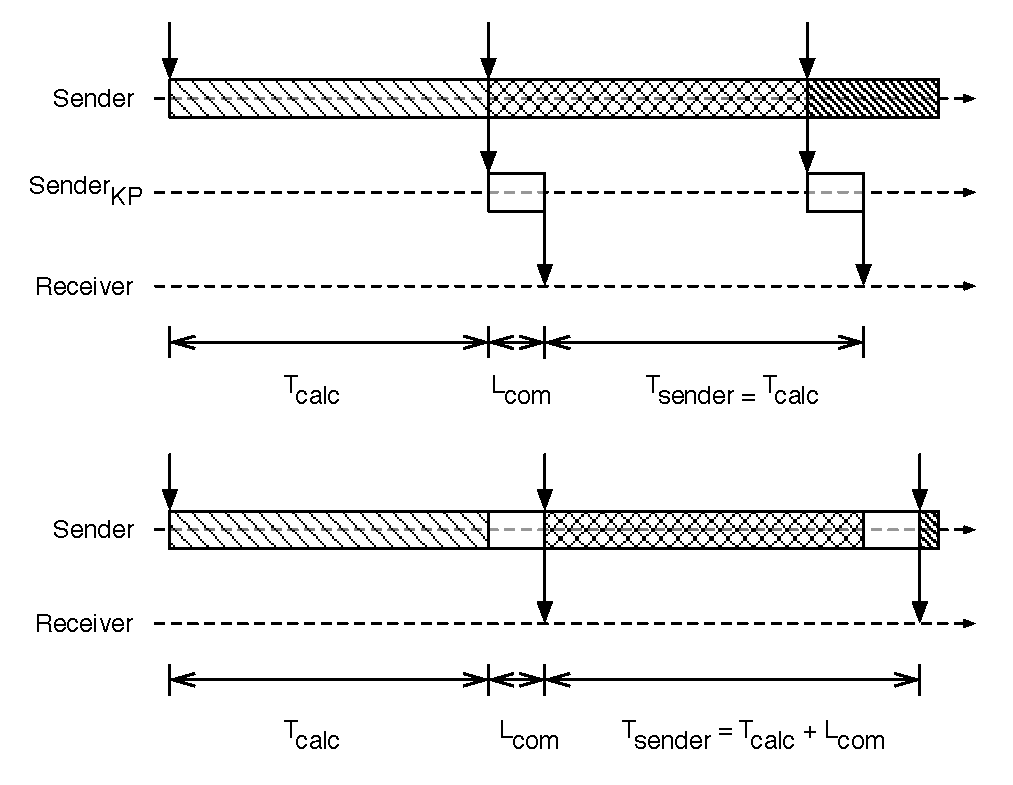
\includegraphics{servicetime_eg_coarse-grain.pdf}}
    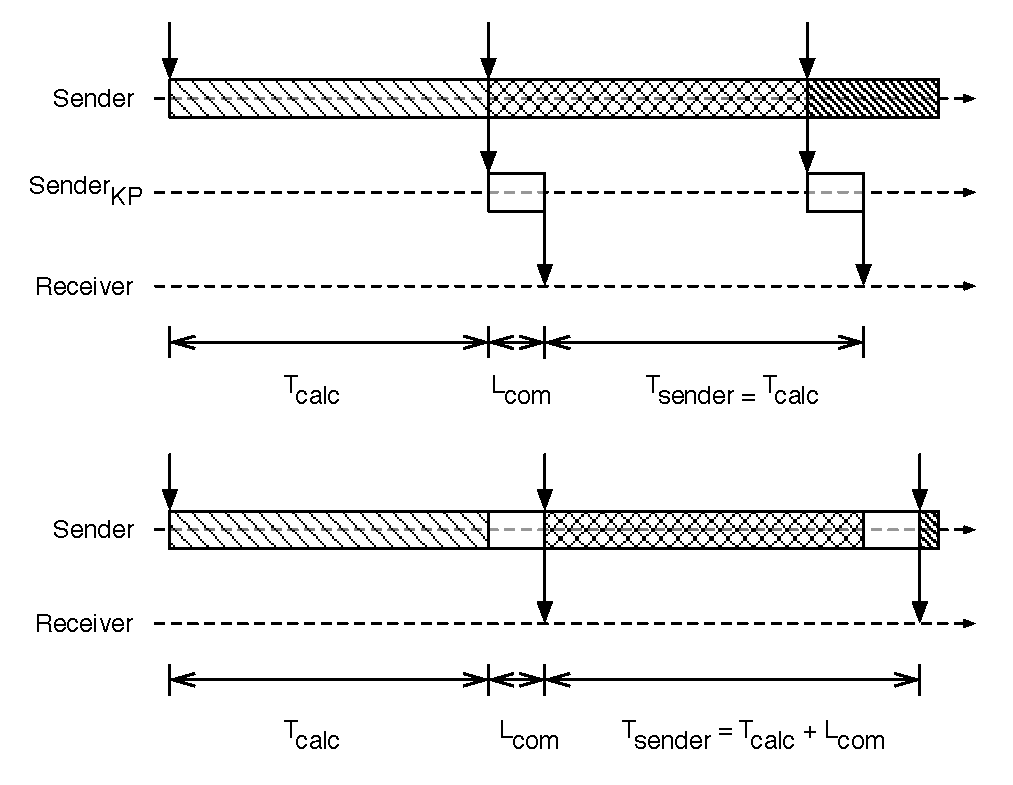
\includegraphics[height=3.0in]{servicetime_eg_coarse-grain.pdf}
  \end{figure}
\end{frame}

\begin{frame}
  \frametitle{Sulla grana del calcolo (2)}
  \note{Talk no more than 1 minute.} 
  \begin{figure}
%    \resizebox{\pageheigth}{!}{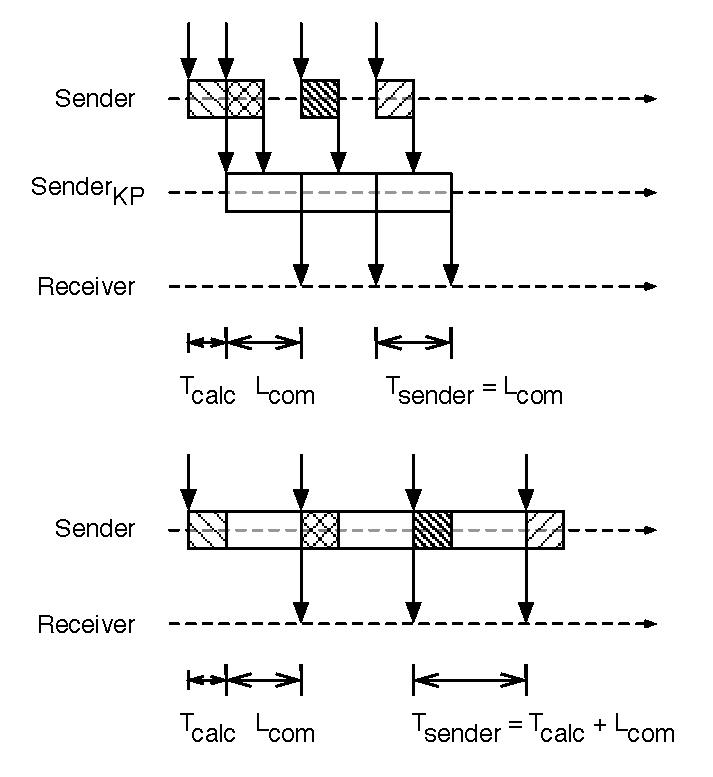
\includegraphics{servicetime_eg_fine-grain.pdf}}
    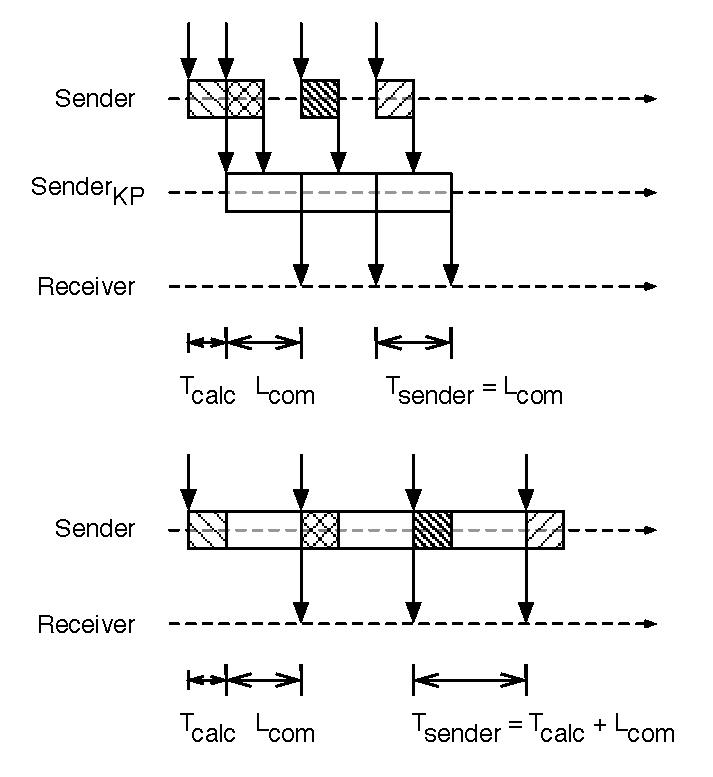
\includegraphics[height=3.0in]{servicetime_eg_fine-grain.pdf}
  \end{figure}
\end{frame}

\begin{frame}
  \frametitle{Forme di comunicazione}
  \begin{columns}
    \column{.5\columnwidth}
    Canale simmetrico
    \column{.5\columnwidth}
    Canale asimmetrico in ingresso
  \end{columns}
  \begin{columns}
    \column{.5\columnwidth}
    \resizebox{\columnwidth}{!}{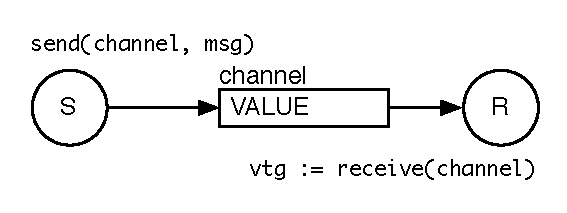
\includegraphics{abstract_sym.pdf}}
    \column{.5\columnwidth}
    \resizebox{\columnwidth}{!}{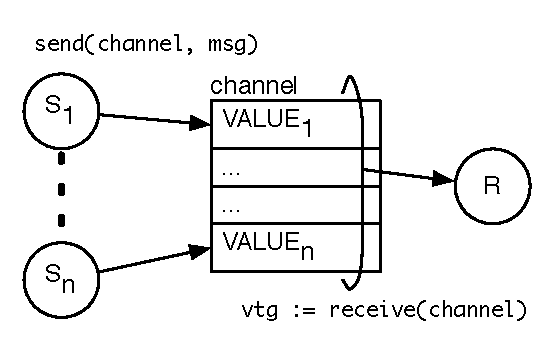
\includegraphics{abstract_asym.pdf}}
  \end{columns}
  \begin{itemize}
    \item Tipo 'riferimento'
    \item Grado asincronia unitario
    \item Semantica Bloccante
    \item Protocollo Rdy-Ack
  \end{itemize}
\end{frame}

\begin{frame}[fragile]
  \frametitle{Implementazioni del canale simmetrico}
  \begin{description}
  \item [uso della Memoria Condivisa] \hfill
    \begin{itemize}
    \item \verb+ch_sym_sm_rdyack_no+ gestione predefinita della coerenza della cache;
    \item \verb+ch_sym_sm_rdyack+ configurazione della coerenza della cache che massimizza la localit\`a delle informazioni del supporto nei core consumatori;
    \item \verb+ch_sym_sm_nullack+ utilizzo di un diverso protocollo di comunicazione che garantisce la correttezza senza l'uso di istruzioni di barriera di memoria
    \end{itemize}
  \item [uso della UDN] \hfill
    \begin{itemize}
    \item \verb+ch_sym_udn+ corrispondenza biunivoca tra i flussi firmware e i canali a livello processi
    \end{itemize}
  \end{description}
\end{frame}

\begin{frame}[fragile]
  \frametitle{Implementazioni del canale simmetrico}
  \begin{description}
  \item [uso della Memoria Condivisa] \hfill
    \begin{itemize}
    \item \verb+ch_asymin_sm_all+ 
    \item \verb+ch_asymin_sm+ 
    \end{itemize}
  \item [uso della UDN] \hfill
    \begin{itemize}
    \item \verb+ch_asymin_udn+ 
    \end{itemize}
  \end{description}
\end{frame}


\section{Esperimenti}

\subsection{Misura della Latenza di comunicazione}

\begin{frame}
  \frametitle{Misura della latenza di comunicazione}
  \begin{itemize}
  \item La latenza di comunicazione \`e misurata per mezzo di una applicazione ``ping-pong'':
    \begin{itemize}
    \item composta da due processi collegati da due canali,
    \item viene svolto lo scambio di $m$ messaggi tra i due processi;
    \end{itemize}
  \item La latenza di comunicazione \`e stimata con $\Lcom = \Tc / (2 \cdot m)$.
  \end{itemize}
  \begin{figure}
    \resizebox{\columnwidth}{!}{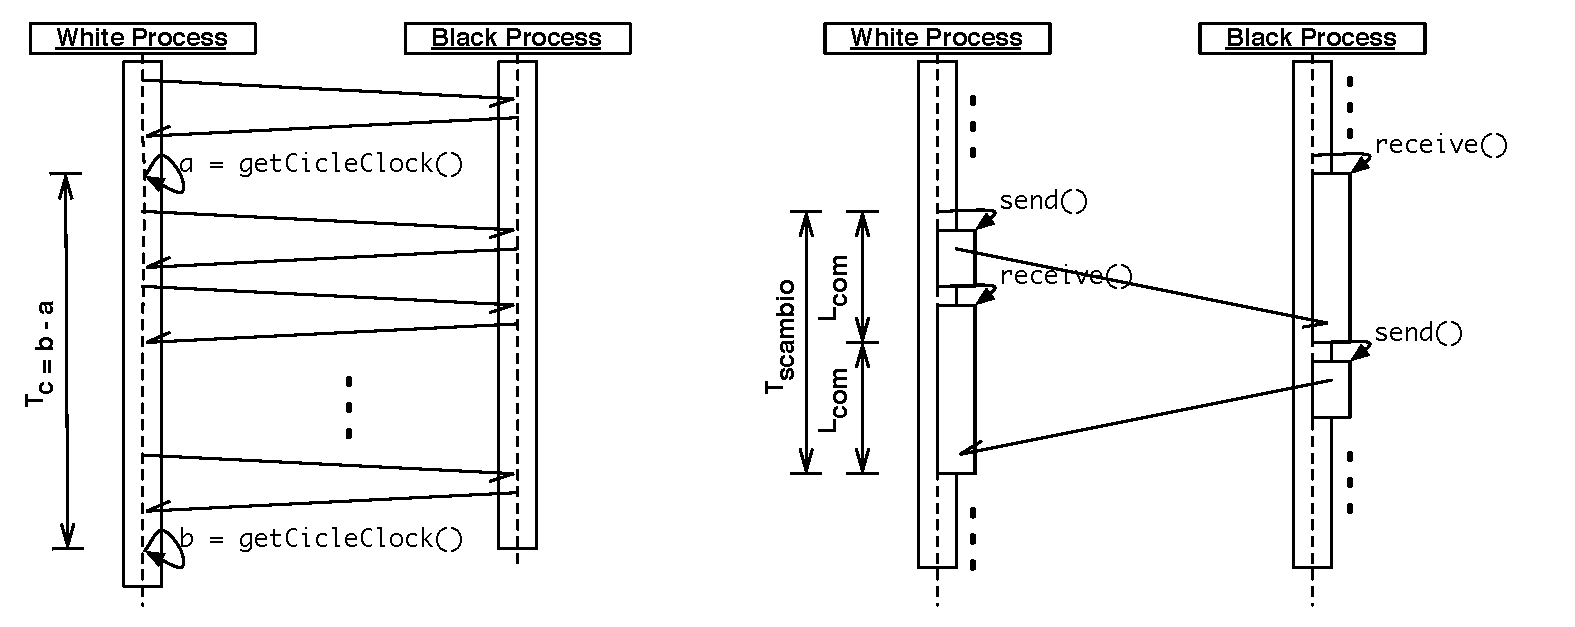
\includegraphics{schema_metering.pdf}}
  \end{figure}
\end{frame}

\begin{frame}
  \frametitle{Misura della latenza del canale simmetrico}
  \begin{figure}
    \resizebox{\columnwidth}{!}{% GNUPLOT: LaTeX picture with Postscript
\begingroup
  \makeatletter
  \providecommand\color[2][]{%
    \GenericError{(gnuplot) \space\space\space\@spaces}{%
      Package color not loaded in conjunction with
      terminal option `colourtext'%
    }{See the gnuplot documentation for explanation.%
    }{Either use 'blacktext' in gnuplot or load the package
      color.sty in LaTeX.}%
    \renewcommand\color[2][]{}%
  }%
  \providecommand\includegraphics[2][]{%
    \GenericError{(gnuplot) \space\space\space\@spaces}{%
      Package graphicx or graphics not loaded%
    }{See the gnuplot documentation for explanation.%
    }{The gnuplot epslatex terminal needs graphicx.sty or graphics.sty.}%
    \renewcommand\includegraphics[2][]{}%
  }%
  \providecommand\rotatebox[2]{#2}%
  \@ifundefined{ifGPcolor}{%
    \newif\ifGPcolor
    \GPcolortrue
  }{}%
  \@ifundefined{ifGPblacktext}{%
    \newif\ifGPblacktext
    \GPblacktexttrue
  }{}%
  % define a \g@addto@macro without @ in the name:
  \let\gplgaddtomacro\g@addto@macro
  % define empty templates for all commands taking text:
  \gdef\gplbacktext{}%
  \gdef\gplfronttext{}%
  \makeatother
  \ifGPblacktext
    % no textcolor at all
    \def\colorrgb#1{}%
    \def\colorgray#1{}%
  \else
    % gray or color?
    \ifGPcolor
      \def\colorrgb#1{\color[rgb]{#1}}%
      \def\colorgray#1{\color[gray]{#1}}%
      \expandafter\def\csname LTw\endcsname{\color{white}}%
      \expandafter\def\csname LTb\endcsname{\color{black}}%
      \expandafter\def\csname LTa\endcsname{\color{black}}%
      \expandafter\def\csname LT0\endcsname{\color[rgb]{1,0,0}}%
      \expandafter\def\csname LT1\endcsname{\color[rgb]{0,1,0}}%
      \expandafter\def\csname LT2\endcsname{\color[rgb]{0,0,1}}%
      \expandafter\def\csname LT3\endcsname{\color[rgb]{1,0,1}}%
      \expandafter\def\csname LT4\endcsname{\color[rgb]{0,1,1}}%
      \expandafter\def\csname LT5\endcsname{\color[rgb]{1,1,0}}%
      \expandafter\def\csname LT6\endcsname{\color[rgb]{0,0,0}}%
      \expandafter\def\csname LT7\endcsname{\color[rgb]{1,0.3,0}}%
      \expandafter\def\csname LT8\endcsname{\color[rgb]{0.5,0.5,0.5}}%
    \else
      % gray
      \def\colorrgb#1{\color{black}}%
      \def\colorgray#1{\color[gray]{#1}}%
      \expandafter\def\csname LTw\endcsname{\color{white}}%
      \expandafter\def\csname LTb\endcsname{\color{black}}%
      \expandafter\def\csname LTa\endcsname{\color{black}}%
      \expandafter\def\csname LT0\endcsname{\color{black}}%
      \expandafter\def\csname LT1\endcsname{\color{black}}%
      \expandafter\def\csname LT2\endcsname{\color{black}}%
      \expandafter\def\csname LT3\endcsname{\color{black}}%
      \expandafter\def\csname LT4\endcsname{\color{black}}%
      \expandafter\def\csname LT5\endcsname{\color{black}}%
      \expandafter\def\csname LT6\endcsname{\color{black}}%
      \expandafter\def\csname LT7\endcsname{\color{black}}%
      \expandafter\def\csname LT8\endcsname{\color{black}}%
    \fi
  \fi
  \setlength{\unitlength}{0.0500bp}%
  \begin{picture}(7200.00,5040.00)%
    \gplgaddtomacro\gplbacktext{%
      \csname LTb\endcsname%
      \put(946,704){\makebox(0,0)[r]{\strut{} 0}}%
      \put(946,1128){\makebox(0,0)[r]{\strut{} 50}}%
      \put(946,1553){\makebox(0,0)[r]{\strut{} 100}}%
      \put(946,1977){\makebox(0,0)[r]{\strut{} 150}}%
      \put(946,2402){\makebox(0,0)[r]{\strut{} 200}}%
      \put(946,2826){\makebox(0,0)[r]{\strut{} 250}}%
      \put(946,3251){\makebox(0,0)[r]{\strut{} 300}}%
      \put(946,3675){\makebox(0,0)[r]{\strut{} 350}}%
      \put(2223,484){\makebox(0,0){\strut{}1}}%
      \put(3369,484){\makebox(0,0){\strut{}8}}%
      \put(4514,484){\makebox(0,0){\strut{}14}}%
      \put(5791,704){\makebox(0,0)[l]{\strut{} 0}}%
      \put(5791,1071){\makebox(0,0)[l]{\strut{} 0.05}}%
      \put(5791,1438){\makebox(0,0)[l]{\strut{} 0.1}}%
      \put(5791,1805){\makebox(0,0)[l]{\strut{} 0.15}}%
      \put(5791,2172){\makebox(0,0)[l]{\strut{} 0.2}}%
      \put(5791,2539){\makebox(0,0)[l]{\strut{} 0.25}}%
      \put(5791,2906){\makebox(0,0)[l]{\strut{} 0.3}}%
      \put(5791,3273){\makebox(0,0)[l]{\strut{} 0.35}}%
      \put(5791,3640){\makebox(0,0)[l]{\strut{} 0.4}}%
      \put(176,2189){\rotatebox{-270}{\makebox(0,0){\strut{}$\mathrm{L}_{\mathrm{com}} \; (\,\tau\,)$}}}%
      \put(6692,2189){\rotatebox{-270}{\makebox(0,0){\strut{}$\mathrm{L}_{\mathrm{com}} \; (\,\mu\mathrm{sec}\,)$}}}%
      \put(3368,154){\makebox(0,0){\strut{}number of hops}}%
    }%
    \gplgaddtomacro\gplfronttext{%
      \csname LTb\endcsname%
      \put(4804,4867){\makebox(0,0)[r]{\strut{}uso della Rete di Interconnessione}}%
      \csname LTb\endcsname%
      \put(4804,4647){\makebox(0,0)[r]{\strut{}uso della Memoria Condivisa, coerenza cache predefinita}}%
      \csname LTb\endcsname%
      \put(4804,4427){\makebox(0,0)[r]{\strut{}uso della SM, configurazione coerenza cache}}%
      \csname LTb\endcsname%
      \put(4804,4207){\makebox(0,0)[r]{\strut{}uso della Memoria Condivisa, non uso di memory barrier}}%
    }%
    \gplbacktext
    \put(0,0){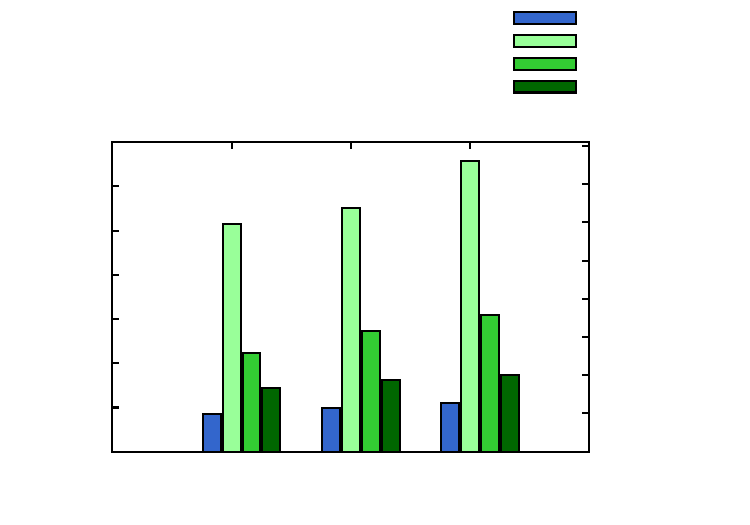
\includegraphics{2_5_sym_all_color}}%
    \gplfronttext
  \end{picture}%
\endgroup
}
  \end{figure}
\end{frame}

\begin{frame}
  \frametitle{Misura della latenza del canale asimmetrico}
  \begin{figure}
    \resizebox{\columnwidth}{!}{% GNUPLOT: LaTeX picture with Postscript
\begingroup
  \makeatletter
  \providecommand\color[2][]{%
    \GenericError{(gnuplot) \space\space\space\@spaces}{%
      Package color not loaded in conjunction with
      terminal option `colourtext'%
    }{See the gnuplot documentation for explanation.%
    }{Either use 'blacktext' in gnuplot or load the package
      color.sty in LaTeX.}%
    \renewcommand\color[2][]{}%
  }%
  \providecommand\includegraphics[2][]{%
    \GenericError{(gnuplot) \space\space\space\@spaces}{%
      Package graphicx or graphics not loaded%
    }{See the gnuplot documentation for explanation.%
    }{The gnuplot epslatex terminal needs graphicx.sty or graphics.sty.}%
    \renewcommand\includegraphics[2][]{}%
  }%
  \providecommand\rotatebox[2]{#2}%
  \@ifundefined{ifGPcolor}{%
    \newif\ifGPcolor
    \GPcolortrue
  }{}%
  \@ifundefined{ifGPblacktext}{%
    \newif\ifGPblacktext
    \GPblacktexttrue
  }{}%
  % define a \g@addto@macro without @ in the name:
  \let\gplgaddtomacro\g@addto@macro
  % define empty templates for all commands taking text:
  \gdef\gplbacktext{}%
  \gdef\gplfronttext{}%
  \makeatother
  \ifGPblacktext
    % no textcolor at all
    \def\colorrgb#1{}%
    \def\colorgray#1{}%
  \else
    % gray or color?
    \ifGPcolor
      \def\colorrgb#1{\color[rgb]{#1}}%
      \def\colorgray#1{\color[gray]{#1}}%
      \expandafter\def\csname LTw\endcsname{\color{white}}%
      \expandafter\def\csname LTb\endcsname{\color{black}}%
      \expandafter\def\csname LTa\endcsname{\color{black}}%
      \expandafter\def\csname LT0\endcsname{\color[rgb]{1,0,0}}%
      \expandafter\def\csname LT1\endcsname{\color[rgb]{0,1,0}}%
      \expandafter\def\csname LT2\endcsname{\color[rgb]{0,0,1}}%
      \expandafter\def\csname LT3\endcsname{\color[rgb]{1,0,1}}%
      \expandafter\def\csname LT4\endcsname{\color[rgb]{0,1,1}}%
      \expandafter\def\csname LT5\endcsname{\color[rgb]{1,1,0}}%
      \expandafter\def\csname LT6\endcsname{\color[rgb]{0,0,0}}%
      \expandafter\def\csname LT7\endcsname{\color[rgb]{1,0.3,0}}%
      \expandafter\def\csname LT8\endcsname{\color[rgb]{0.5,0.5,0.5}}%
    \else
      % gray
      \def\colorrgb#1{\color{black}}%
      \def\colorgray#1{\color[gray]{#1}}%
      \expandafter\def\csname LTw\endcsname{\color{white}}%
      \expandafter\def\csname LTb\endcsname{\color{black}}%
      \expandafter\def\csname LTa\endcsname{\color{black}}%
      \expandafter\def\csname LT0\endcsname{\color{black}}%
      \expandafter\def\csname LT1\endcsname{\color{black}}%
      \expandafter\def\csname LT2\endcsname{\color{black}}%
      \expandafter\def\csname LT3\endcsname{\color{black}}%
      \expandafter\def\csname LT4\endcsname{\color{black}}%
      \expandafter\def\csname LT5\endcsname{\color{black}}%
      \expandafter\def\csname LT6\endcsname{\color{black}}%
      \expandafter\def\csname LT7\endcsname{\color{black}}%
      \expandafter\def\csname LT8\endcsname{\color{black}}%
    \fi
  \fi
  \setlength{\unitlength}{0.0500bp}%
  \begin{picture}(7200.00,5040.00)%
    \gplgaddtomacro\gplbacktext{%
      \csname LTb\endcsname%
      \put(946,704){\makebox(0,0)[r]{\strut{} 0}}%
      \put(946,1059){\makebox(0,0)[r]{\strut{} 50}}%
      \put(946,1413){\makebox(0,0)[r]{\strut{} 100}}%
      \put(946,1768){\makebox(0,0)[r]{\strut{} 150}}%
      \put(946,2122){\makebox(0,0)[r]{\strut{} 200}}%
      \put(946,2477){\makebox(0,0)[r]{\strut{} 250}}%
      \put(946,2831){\makebox(0,0)[r]{\strut{} 300}}%
      \put(946,3186){\makebox(0,0)[r]{\strut{} 350}}%
      \put(946,3540){\makebox(0,0)[r]{\strut{} 400}}%
      \put(946,3895){\makebox(0,0)[r]{\strut{} 450}}%
      \put(2256,484){\makebox(0,0){\strut{}1}}%
      \put(3435,484){\makebox(0,0){\strut{}8}}%
      \put(4613,484){\makebox(0,0){\strut{}14}}%
      \put(5923,704){\makebox(0,0)[l]{\strut{} 0}}%
      \put(5923,1317){\makebox(0,0)[l]{\strut{} 0.1}}%
      \put(5923,1930){\makebox(0,0)[l]{\strut{} 0.2}}%
      \put(5923,2543){\makebox(0,0)[l]{\strut{} 0.3}}%
      \put(5923,3156){\makebox(0,0)[l]{\strut{} 0.4}}%
      \put(5923,3769){\makebox(0,0)[l]{\strut{} 0.5}}%
      \put(176,2299){\rotatebox{-270}{\makebox(0,0){\strut{}$\mathrm{L}_{\mathrm{com}} \; (\,\tau\,)$}}}%
      \put(6692,2299){\rotatebox{-270}{\makebox(0,0){\strut{}$\mathrm{L}_{\mathrm{com}} \; (\,\mu\mathrm{sec}\,)$}}}%
      \put(3434,154){\makebox(0,0){\strut{}number of hops}}%
    }%
    \gplgaddtomacro\gplfronttext{%
      \csname LTb\endcsname%
      \put(4936,4867){\makebox(0,0)[r]{\strut{}uso della Rete di Interconnessione}}%
      \csname LTb\endcsname%
      \put(4936,4647){\makebox(0,0)[r]{\strut{}uso della memoria condivisa, allocati tutti i mittenti}}%
      \csname LTb\endcsname%
      \put(4936,4427){\makebox(0,0)[r]{\strut{}uso della memoria condivisa, allocato un unico mittente}}%
    }%
    \gplbacktext
    \put(0,0){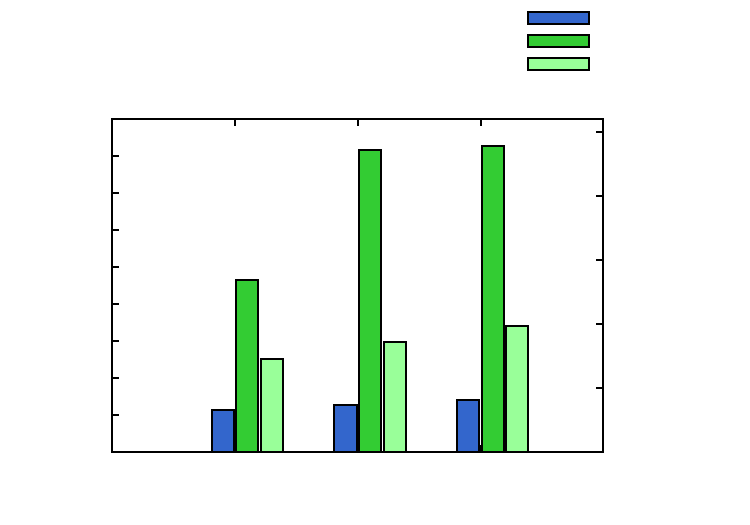
\includegraphics{2_5_asymin_all_color}}%
    \gplfronttext
  \end{picture}%
\endgroup
}
  \end{figure}
\end{frame}

\subsection{Benchmark}

\begin{frame}
  \frametitle{Benchmark: prodotto matrice-vettore su stream}
  \[ \mathbf{A} = (a_{ij})_{i=1,\ldots,\mathrm{M}, j=1,\ldots,\mathrm{M}} \in \mathbb{Z}^{\mathrm{MxM}} \]
  \[ \mathbf{b} = (b_1,\ldots,b_\mathrm{M}) \in \mathbb{Z}^{\mathrm{M}} \]
  \[ \mathbf{c} = (c_1,\ldots,c_\mathrm{M}) = \mathbf{A} \cdot \mathbf{b} \in \mathbb{Z}^{\mathrm{M}} \]
  \[ \forall \; i \in \{1,\ldots,\mathrm{M}\} \; : \; c_i = \mathbf{a}_i \cdot \mathbf{b} = \sum_{j=1}^{\mathrm{M}} a_{ij} \cdot b_j  \]
  
  \begin{figure}
    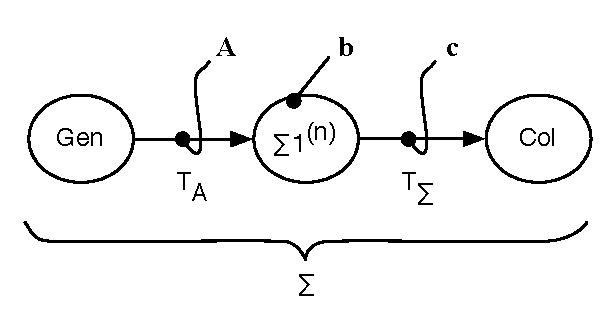
\includegraphics[scale=.5]{grafo_sigma_compatto.pdf}
  \end{figure}
\end{frame}


\note{Si basa sul partizionamento dei dati in ingresso e sulla replicazione della funzione di calcolo nelle unit\`a worker.}

\begin{frame}
  \frametitle{Benchmark: soluzione parallela}
  \begin{columns}[c]
    \column{.5\textwidth}
    \begin{itemize}
\item Data Parallel Map
\item Multicast strutturata ad albero distribuito nei worker
\end{itemize}
    \column{.5\textwidth} 
  \begin{figure}
    \resizebox{.90\columnwidth}{!}{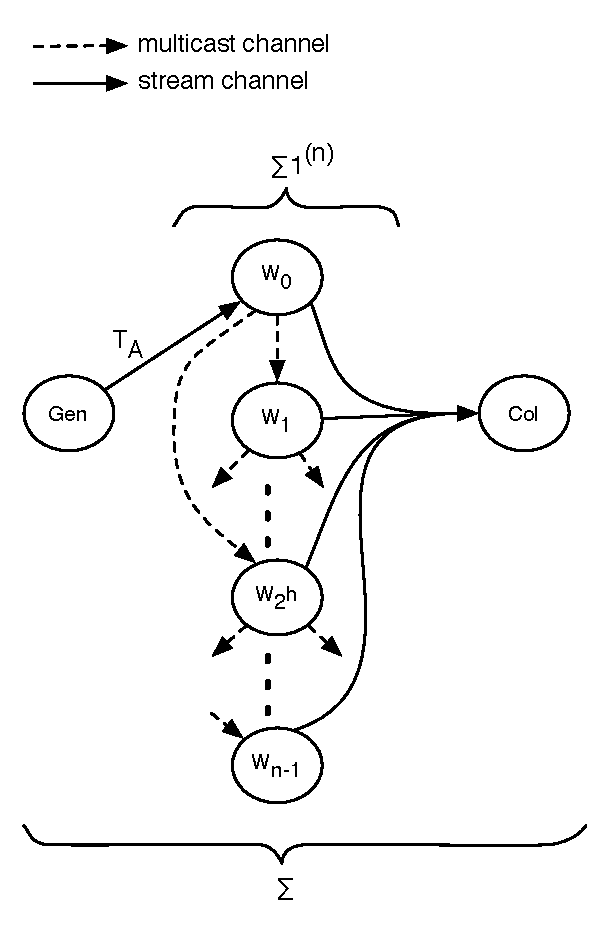
\includegraphics{grafo_sigma_vert.pdf}}
  \end{figure}  

  \end{columns}
\end{frame}

\begin{frame}
  \frametitle{Confronto: tempo di servizio (1)}
  \begin{itemize}
  \item Tempo di interarrivo 4.627 \musec
  \item Dimensione delle matrici 56x56
  \item Tempo di servizio migliore UDN ... Tempo di servizio migliore SM ...
  \end{itemize}
  \begin{columns}
    \column{.5\columnwidth}
    \resizebox{\columnwidth}{!}{% GNUPLOT: LaTeX picture with Postscript
\begingroup
  \makeatletter
  \providecommand\color[2][]{%
    \GenericError{(gnuplot) \space\space\space\@spaces}{%
      Package color not loaded in conjunction with
      terminal option `colourtext'%
    }{See the gnuplot documentation for explanation.%
    }{Either use 'blacktext' in gnuplot or load the package
      color.sty in LaTeX.}%
    \renewcommand\color[2][]{}%
  }%
  \providecommand\includegraphics[2][]{%
    \GenericError{(gnuplot) \space\space\space\@spaces}{%
      Package graphicx or graphics not loaded%
    }{See the gnuplot documentation for explanation.%
    }{The gnuplot epslatex terminal needs graphicx.sty or graphics.sty.}%
    \renewcommand\includegraphics[2][]{}%
  }%
  \providecommand\rotatebox[2]{#2}%
  \@ifundefined{ifGPcolor}{%
    \newif\ifGPcolor
    \GPcolortrue
  }{}%
  \@ifundefined{ifGPblacktext}{%
    \newif\ifGPblacktext
    \GPblacktexttrue
  }{}%
  % define a \g@addto@macro without @ in the name:
  \let\gplgaddtomacro\g@addto@macro
  % define empty templates for all commands taking text:
  \gdef\gplbacktext{}%
  \gdef\gplfronttext{}%
  \makeatother
  \ifGPblacktext
    % no textcolor at all
    \def\colorrgb#1{}%
    \def\colorgray#1{}%
  \else
    % gray or color?
    \ifGPcolor
      \def\colorrgb#1{\color[rgb]{#1}}%
      \def\colorgray#1{\color[gray]{#1}}%
      \expandafter\def\csname LTw\endcsname{\color{white}}%
      \expandafter\def\csname LTb\endcsname{\color{black}}%
      \expandafter\def\csname LTa\endcsname{\color{black}}%
      \expandafter\def\csname LT0\endcsname{\color[rgb]{1,0,0}}%
      \expandafter\def\csname LT1\endcsname{\color[rgb]{0,1,0}}%
      \expandafter\def\csname LT2\endcsname{\color[rgb]{0,0,1}}%
      \expandafter\def\csname LT3\endcsname{\color[rgb]{1,0,1}}%
      \expandafter\def\csname LT4\endcsname{\color[rgb]{0,1,1}}%
      \expandafter\def\csname LT5\endcsname{\color[rgb]{1,1,0}}%
      \expandafter\def\csname LT6\endcsname{\color[rgb]{0,0,0}}%
      \expandafter\def\csname LT7\endcsname{\color[rgb]{1,0.3,0}}%
      \expandafter\def\csname LT8\endcsname{\color[rgb]{0.5,0.5,0.5}}%
    \else
      % gray
      \def\colorrgb#1{\color{black}}%
      \def\colorgray#1{\color[gray]{#1}}%
      \expandafter\def\csname LTw\endcsname{\color{white}}%
      \expandafter\def\csname LTb\endcsname{\color{black}}%
      \expandafter\def\csname LTa\endcsname{\color{black}}%
      \expandafter\def\csname LT0\endcsname{\color{black}}%
      \expandafter\def\csname LT1\endcsname{\color{black}}%
      \expandafter\def\csname LT2\endcsname{\color{black}}%
      \expandafter\def\csname LT3\endcsname{\color{black}}%
      \expandafter\def\csname LT4\endcsname{\color{black}}%
      \expandafter\def\csname LT5\endcsname{\color{black}}%
      \expandafter\def\csname LT6\endcsname{\color{black}}%
      \expandafter\def\csname LT7\endcsname{\color{black}}%
      \expandafter\def\csname LT8\endcsname{\color{black}}%
    \fi
  \fi
  \setlength{\unitlength}{0.0500bp}%
  \begin{picture}(7200.00,5040.00)%
    \gplgaddtomacro\gplbacktext{%
      \csname LTb\endcsname%
      \put(814,1325){\makebox(0,0)[r]{\strut{} 10}}%
      \csname LTb\endcsname%
      \put(814,2015){\makebox(0,0)[r]{\strut{} 20}}%
      \csname LTb\endcsname%
      \put(814,2705){\makebox(0,0)[r]{\strut{} 30}}%
      \csname LTb\endcsname%
      \put(814,3395){\makebox(0,0)[r]{\strut{} 40}}%
      \csname LTb\endcsname%
      \put(814,4085){\makebox(0,0)[r]{\strut{} 50}}%
      \csname LTb\endcsname%
      \put(814,4775){\makebox(0,0)[r]{\strut{} 60}}%
      \csname LTb\endcsname%
      \put(1839,484){\makebox(0,0){\strut{} 10}}%
      \csname LTb\endcsname%
      \put(2832,484){\makebox(0,0){\strut{} 20}}%
      \csname LTb\endcsname%
      \put(3825,484){\makebox(0,0){\strut{} 30}}%
      \csname LTb\endcsname%
      \put(4818,484){\makebox(0,0){\strut{} 40}}%
      \csname LTb\endcsname%
      \put(5810,484){\makebox(0,0){\strut{} 50}}%
      \csname LTb\endcsname%
      \put(6803,484){\makebox(0,0){\strut{} 60}}%
      \put(176,2739){\rotatebox{-270}{\makebox(0,0){\strut{}scalability}}}%
      \put(3874,154){\makebox(0,0){\strut{}$n$ parallel degree}}%
    }%
    \gplgaddtomacro\gplfronttext{%
      \csname LTb\endcsname%
      \put(3322,4602){\makebox(0,0)[r]{\strut{}ideal scalability}}%
      \csname LTb\endcsname%
      \put(3322,4382){\makebox(0,0)[r]{\strut{}udn udn}}%
      \csname LTb\endcsname%
      \put(3322,4162){\makebox(0,0)[r]{\strut{}sm sm}}%
    }%
    \gplbacktext
    \put(0,0){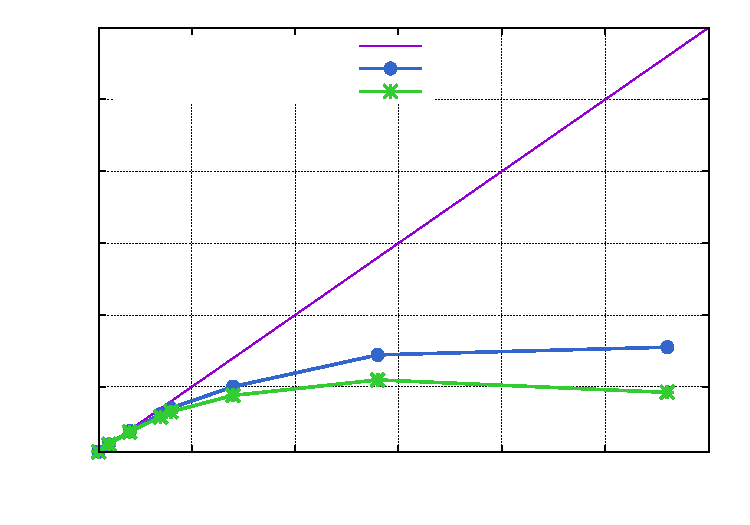
\includegraphics{plot-comp-T-s_nogatherInt_selected_500_4000_56_slide}}%
    \gplfronttext
  \end{picture}%
\endgroup
}
    \column{.5\columnwidth}
    \resizebox{\columnwidth}{!}{% GNUPLOT: LaTeX picture with Postscript
\begingroup
  \makeatletter
  \providecommand\color[2][]{%
    \GenericError{(gnuplot) \space\space\space\@spaces}{%
      Package color not loaded in conjunction with
      terminal option `colourtext'%
    }{See the gnuplot documentation for explanation.%
    }{Either use 'blacktext' in gnuplot or load the package
      color.sty in LaTeX.}%
    \renewcommand\color[2][]{}%
  }%
  \providecommand\includegraphics[2][]{%
    \GenericError{(gnuplot) \space\space\space\@spaces}{%
      Package graphicx or graphics not loaded%
    }{See the gnuplot documentation for explanation.%
    }{The gnuplot epslatex terminal needs graphicx.sty or graphics.sty.}%
    \renewcommand\includegraphics[2][]{}%
  }%
  \providecommand\rotatebox[2]{#2}%
  \@ifundefined{ifGPcolor}{%
    \newif\ifGPcolor
    \GPcolortrue
  }{}%
  \@ifundefined{ifGPblacktext}{%
    \newif\ifGPblacktext
    \GPblacktexttrue
  }{}%
  % define a \g@addto@macro without @ in the name:
  \let\gplgaddtomacro\g@addto@macro
  % define empty templates for all commands taking text:
  \gdef\gplbacktext{}%
  \gdef\gplfronttext{}%
  \makeatother
  \ifGPblacktext
    % no textcolor at all
    \def\colorrgb#1{}%
    \def\colorgray#1{}%
  \else
    % gray or color?
    \ifGPcolor
      \def\colorrgb#1{\color[rgb]{#1}}%
      \def\colorgray#1{\color[gray]{#1}}%
      \expandafter\def\csname LTw\endcsname{\color{white}}%
      \expandafter\def\csname LTb\endcsname{\color{black}}%
      \expandafter\def\csname LTa\endcsname{\color{black}}%
      \expandafter\def\csname LT0\endcsname{\color[rgb]{1,0,0}}%
      \expandafter\def\csname LT1\endcsname{\color[rgb]{0,1,0}}%
      \expandafter\def\csname LT2\endcsname{\color[rgb]{0,0,1}}%
      \expandafter\def\csname LT3\endcsname{\color[rgb]{1,0,1}}%
      \expandafter\def\csname LT4\endcsname{\color[rgb]{0,1,1}}%
      \expandafter\def\csname LT5\endcsname{\color[rgb]{1,1,0}}%
      \expandafter\def\csname LT6\endcsname{\color[rgb]{0,0,0}}%
      \expandafter\def\csname LT7\endcsname{\color[rgb]{1,0.3,0}}%
      \expandafter\def\csname LT8\endcsname{\color[rgb]{0.5,0.5,0.5}}%
    \else
      % gray
      \def\colorrgb#1{\color{black}}%
      \def\colorgray#1{\color[gray]{#1}}%
      \expandafter\def\csname LTw\endcsname{\color{white}}%
      \expandafter\def\csname LTb\endcsname{\color{black}}%
      \expandafter\def\csname LTa\endcsname{\color{black}}%
      \expandafter\def\csname LT0\endcsname{\color{black}}%
      \expandafter\def\csname LT1\endcsname{\color{black}}%
      \expandafter\def\csname LT2\endcsname{\color{black}}%
      \expandafter\def\csname LT3\endcsname{\color{black}}%
      \expandafter\def\csname LT4\endcsname{\color{black}}%
      \expandafter\def\csname LT5\endcsname{\color{black}}%
      \expandafter\def\csname LT6\endcsname{\color{black}}%
      \expandafter\def\csname LT7\endcsname{\color{black}}%
      \expandafter\def\csname LT8\endcsname{\color{black}}%
    \fi
  \fi
  \setlength{\unitlength}{0.0500bp}%
  \begin{picture}(7200.00,5040.00)%
    \gplgaddtomacro\gplbacktext{%
      \csname LTb\endcsname%
      \put(946,704){\makebox(0,0)[r]{\strut{} 1}}%
      \csname LTb\endcsname%
      \put(946,2740){\makebox(0,0)[r]{\strut{} 10}}%
      \csname LTb\endcsname%
      \put(946,4775){\makebox(0,0)[r]{\strut{} 100}}%
      \csname LTb\endcsname%
      \put(1951,484){\makebox(0,0){\strut{} 10}}%
      \csname LTb\endcsname%
      \put(2922,484){\makebox(0,0){\strut{} 20}}%
      \csname LTb\endcsname%
      \put(3892,484){\makebox(0,0){\strut{} 30}}%
      \csname LTb\endcsname%
      \put(4862,484){\makebox(0,0){\strut{} 40}}%
      \csname LTb\endcsname%
      \put(5833,484){\makebox(0,0){\strut{} 50}}%
      \csname LTb\endcsname%
      \put(6803,484){\makebox(0,0){\strut{} 60}}%
      \put(176,2739){\rotatebox{-270}{\makebox(0,0){\strut{}service time ($\,\mu\mathrm{sec}$\,)}}}%
      \put(3940,154){\makebox(0,0){\strut{}$n$ parallel degree}}%
    }%
    \gplgaddtomacro\gplfronttext{%
      \csname LTb\endcsname%
      \put(3586,4602){\makebox(0,0)[r]{\strut{}ideal service time}}%
      \csname LTb\endcsname%
      \put(3586,4382){\makebox(0,0)[r]{\strut{}udn udn}}%
      \csname LTb\endcsname%
      \put(3586,4162){\makebox(0,0)[r]{\strut{}sm sm}}%
    }%
    \gplbacktext
    \put(0,0){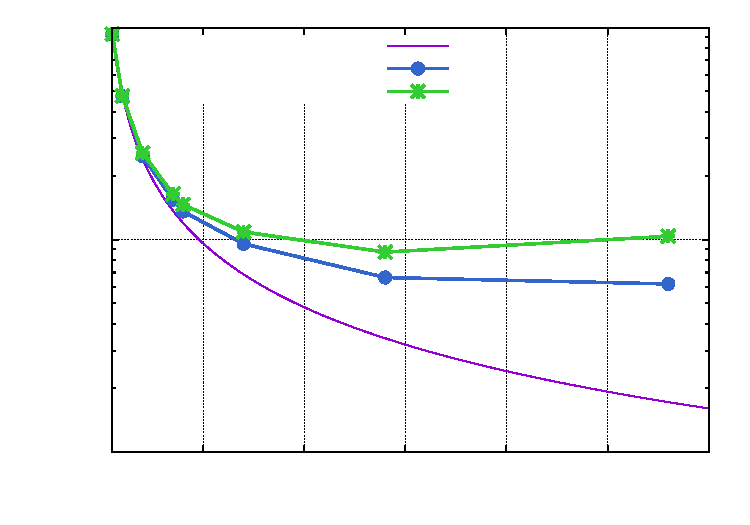
\includegraphics{plot-T-UDN-SM_nogatherInt_selected_500_selected_56_slide}}%
    \gplfronttext
  \end{picture}%
\endgroup
}
  \end{columns}
\end{frame}

\begin{frame}
  \frametitle{Confronto: tempo di servizio (2)}
  \begin{itemize}
  \item Tempo di interarrivo 4.627 \musec %23.133 \musec
  \item Dimensione delle matrici 168x168
  \end{itemize}
  \begin{columns}
    \column{.5\columnwidth}
    \resizebox{\columnwidth}{!}{% GNUPLOT: LaTeX picture with Postscript
\begingroup
  \makeatletter
  \providecommand\color[2][]{%
    \GenericError{(gnuplot) \space\space\space\@spaces}{%
      Package color not loaded in conjunction with
      terminal option `colourtext'%
    }{See the gnuplot documentation for explanation.%
    }{Either use 'blacktext' in gnuplot or load the package
      color.sty in LaTeX.}%
    \renewcommand\color[2][]{}%
  }%
  \providecommand\includegraphics[2][]{%
    \GenericError{(gnuplot) \space\space\space\@spaces}{%
      Package graphicx or graphics not loaded%
    }{See the gnuplot documentation for explanation.%
    }{The gnuplot epslatex terminal needs graphicx.sty or graphics.sty.}%
    \renewcommand\includegraphics[2][]{}%
  }%
  \providecommand\rotatebox[2]{#2}%
  \@ifundefined{ifGPcolor}{%
    \newif\ifGPcolor
    \GPcolortrue
  }{}%
  \@ifundefined{ifGPblacktext}{%
    \newif\ifGPblacktext
    \GPblacktexttrue
  }{}%
  % define a \g@addto@macro without @ in the name:
  \let\gplgaddtomacro\g@addto@macro
  % define empty templates for all commands taking text:
  \gdef\gplbacktext{}%
  \gdef\gplfronttext{}%
  \makeatother
  \ifGPblacktext
    % no textcolor at all
    \def\colorrgb#1{}%
    \def\colorgray#1{}%
  \else
    % gray or color?
    \ifGPcolor
      \def\colorrgb#1{\color[rgb]{#1}}%
      \def\colorgray#1{\color[gray]{#1}}%
      \expandafter\def\csname LTw\endcsname{\color{white}}%
      \expandafter\def\csname LTb\endcsname{\color{black}}%
      \expandafter\def\csname LTa\endcsname{\color{black}}%
      \expandafter\def\csname LT0\endcsname{\color[rgb]{1,0,0}}%
      \expandafter\def\csname LT1\endcsname{\color[rgb]{0,1,0}}%
      \expandafter\def\csname LT2\endcsname{\color[rgb]{0,0,1}}%
      \expandafter\def\csname LT3\endcsname{\color[rgb]{1,0,1}}%
      \expandafter\def\csname LT4\endcsname{\color[rgb]{0,1,1}}%
      \expandafter\def\csname LT5\endcsname{\color[rgb]{1,1,0}}%
      \expandafter\def\csname LT6\endcsname{\color[rgb]{0,0,0}}%
      \expandafter\def\csname LT7\endcsname{\color[rgb]{1,0.3,0}}%
      \expandafter\def\csname LT8\endcsname{\color[rgb]{0.5,0.5,0.5}}%
    \else
      % gray
      \def\colorrgb#1{\color{black}}%
      \def\colorgray#1{\color[gray]{#1}}%
      \expandafter\def\csname LTw\endcsname{\color{white}}%
      \expandafter\def\csname LTb\endcsname{\color{black}}%
      \expandafter\def\csname LTa\endcsname{\color{black}}%
      \expandafter\def\csname LT0\endcsname{\color{black}}%
      \expandafter\def\csname LT1\endcsname{\color{black}}%
      \expandafter\def\csname LT2\endcsname{\color{black}}%
      \expandafter\def\csname LT3\endcsname{\color{black}}%
      \expandafter\def\csname LT4\endcsname{\color{black}}%
      \expandafter\def\csname LT5\endcsname{\color{black}}%
      \expandafter\def\csname LT6\endcsname{\color{black}}%
      \expandafter\def\csname LT7\endcsname{\color{black}}%
      \expandafter\def\csname LT8\endcsname{\color{black}}%
    \fi
  \fi
  \setlength{\unitlength}{0.0500bp}%
  \begin{picture}(7200.00,5040.00)%
    \gplgaddtomacro\gplbacktext{%
      \csname LTb\endcsname%
      \put(814,1325){\makebox(0,0)[r]{\strut{} 10}}%
      \csname LTb\endcsname%
      \put(814,2015){\makebox(0,0)[r]{\strut{} 20}}%
      \csname LTb\endcsname%
      \put(814,2705){\makebox(0,0)[r]{\strut{} 30}}%
      \csname LTb\endcsname%
      \put(814,3395){\makebox(0,0)[r]{\strut{} 40}}%
      \csname LTb\endcsname%
      \put(814,4085){\makebox(0,0)[r]{\strut{} 50}}%
      \csname LTb\endcsname%
      \put(814,4775){\makebox(0,0)[r]{\strut{} 60}}%
      \csname LTb\endcsname%
      \put(1839,484){\makebox(0,0){\strut{} 10}}%
      \csname LTb\endcsname%
      \put(2832,484){\makebox(0,0){\strut{} 20}}%
      \csname LTb\endcsname%
      \put(3825,484){\makebox(0,0){\strut{} 30}}%
      \csname LTb\endcsname%
      \put(4818,484){\makebox(0,0){\strut{} 40}}%
      \csname LTb\endcsname%
      \put(5810,484){\makebox(0,0){\strut{} 50}}%
      \csname LTb\endcsname%
      \put(6803,484){\makebox(0,0){\strut{} 60}}%
      \put(176,2739){\rotatebox{-270}{\makebox(0,0){\strut{}scalability}}}%
      \put(3874,154){\makebox(0,0){\strut{}$n$ parallel degree}}%
    }%
    \gplgaddtomacro\gplfronttext{%
      \csname LTb\endcsname%
      \put(3322,4602){\makebox(0,0)[r]{\strut{}ideal scalability}}%
      \csname LTb\endcsname%
      \put(3322,4382){\makebox(0,0)[r]{\strut{}udn udn}}%
      \csname LTb\endcsname%
      \put(3322,4162){\makebox(0,0)[r]{\strut{}sm sm}}%
    }%
    \gplbacktext
    \put(0,0){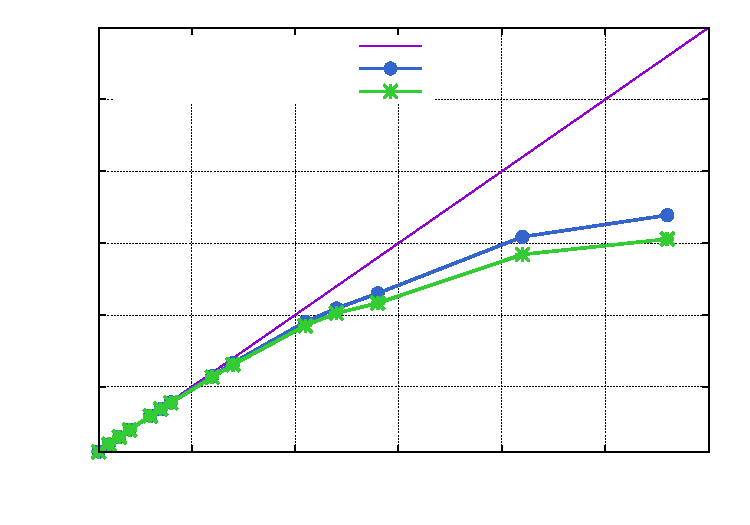
\includegraphics{plot-comp-T-s_nogatherInt_selected_500_20000_168_slide}}%
    \gplfronttext
  \end{picture}%
\endgroup
}
    \column{.5\columnwidth}
    \resizebox{\columnwidth}{!}{% GNUPLOT: LaTeX picture with Postscript
\begingroup
  \makeatletter
  \providecommand\color[2][]{%
    \GenericError{(gnuplot) \space\space\space\@spaces}{%
      Package color not loaded in conjunction with
      terminal option `colourtext'%
    }{See the gnuplot documentation for explanation.%
    }{Either use 'blacktext' in gnuplot or load the package
      color.sty in LaTeX.}%
    \renewcommand\color[2][]{}%
  }%
  \providecommand\includegraphics[2][]{%
    \GenericError{(gnuplot) \space\space\space\@spaces}{%
      Package graphicx or graphics not loaded%
    }{See the gnuplot documentation for explanation.%
    }{The gnuplot epslatex terminal needs graphicx.sty or graphics.sty.}%
    \renewcommand\includegraphics[2][]{}%
  }%
  \providecommand\rotatebox[2]{#2}%
  \@ifundefined{ifGPcolor}{%
    \newif\ifGPcolor
    \GPcolortrue
  }{}%
  \@ifundefined{ifGPblacktext}{%
    \newif\ifGPblacktext
    \GPblacktexttrue
  }{}%
  % define a \g@addto@macro without @ in the name:
  \let\gplgaddtomacro\g@addto@macro
  % define empty templates for all commands taking text:
  \gdef\gplbacktext{}%
  \gdef\gplfronttext{}%
  \makeatother
  \ifGPblacktext
    % no textcolor at all
    \def\colorrgb#1{}%
    \def\colorgray#1{}%
  \else
    % gray or color?
    \ifGPcolor
      \def\colorrgb#1{\color[rgb]{#1}}%
      \def\colorgray#1{\color[gray]{#1}}%
      \expandafter\def\csname LTw\endcsname{\color{white}}%
      \expandafter\def\csname LTb\endcsname{\color{black}}%
      \expandafter\def\csname LTa\endcsname{\color{black}}%
      \expandafter\def\csname LT0\endcsname{\color[rgb]{1,0,0}}%
      \expandafter\def\csname LT1\endcsname{\color[rgb]{0,1,0}}%
      \expandafter\def\csname LT2\endcsname{\color[rgb]{0,0,1}}%
      \expandafter\def\csname LT3\endcsname{\color[rgb]{1,0,1}}%
      \expandafter\def\csname LT4\endcsname{\color[rgb]{0,1,1}}%
      \expandafter\def\csname LT5\endcsname{\color[rgb]{1,1,0}}%
      \expandafter\def\csname LT6\endcsname{\color[rgb]{0,0,0}}%
      \expandafter\def\csname LT7\endcsname{\color[rgb]{1,0.3,0}}%
      \expandafter\def\csname LT8\endcsname{\color[rgb]{0.5,0.5,0.5}}%
    \else
      % gray
      \def\colorrgb#1{\color{black}}%
      \def\colorgray#1{\color[gray]{#1}}%
      \expandafter\def\csname LTw\endcsname{\color{white}}%
      \expandafter\def\csname LTb\endcsname{\color{black}}%
      \expandafter\def\csname LTa\endcsname{\color{black}}%
      \expandafter\def\csname LT0\endcsname{\color{black}}%
      \expandafter\def\csname LT1\endcsname{\color{black}}%
      \expandafter\def\csname LT2\endcsname{\color{black}}%
      \expandafter\def\csname LT3\endcsname{\color{black}}%
      \expandafter\def\csname LT4\endcsname{\color{black}}%
      \expandafter\def\csname LT5\endcsname{\color{black}}%
      \expandafter\def\csname LT6\endcsname{\color{black}}%
      \expandafter\def\csname LT7\endcsname{\color{black}}%
      \expandafter\def\csname LT8\endcsname{\color{black}}%
    \fi
  \fi
  \setlength{\unitlength}{0.0500bp}%
  \begin{picture}(7200.00,5040.00)%
    \gplgaddtomacro\gplbacktext{%
      \csname LTb\endcsname%
      \put(1078,704){\makebox(0,0)[r]{\strut{} 10}}%
      \csname LTb\endcsname%
      \put(1078,2740){\makebox(0,0)[r]{\strut{} 100}}%
      \csname LTb\endcsname%
      \put(1078,4775){\makebox(0,0)[r]{\strut{} 1000}}%
      \csname LTb\endcsname%
      \put(2063,484){\makebox(0,0){\strut{} 10}}%
      \csname LTb\endcsname%
      \put(3011,484){\makebox(0,0){\strut{} 20}}%
      \csname LTb\endcsname%
      \put(3959,484){\makebox(0,0){\strut{} 30}}%
      \csname LTb\endcsname%
      \put(4907,484){\makebox(0,0){\strut{} 40}}%
      \csname LTb\endcsname%
      \put(5855,484){\makebox(0,0){\strut{} 50}}%
      \csname LTb\endcsname%
      \put(6803,484){\makebox(0,0){\strut{} 60}}%
      \put(176,2739){\rotatebox{-270}{\makebox(0,0){\strut{}service time ($\,\mu\mathrm{sec}$\,)}}}%
      \put(4006,154){\makebox(0,0){\strut{}$n$ parallel degree}}%
    }%
    \gplgaddtomacro\gplfronttext{%
      \csname LTb\endcsname%
      \put(3718,4602){\makebox(0,0)[r]{\strut{}ideal service time}}%
      \csname LTb\endcsname%
      \put(3718,4382){\makebox(0,0)[r]{\strut{}udn udn}}%
      \csname LTb\endcsname%
      \put(3718,4162){\makebox(0,0)[r]{\strut{}sm sm}}%
    }%
    \gplbacktext
    \put(0,0){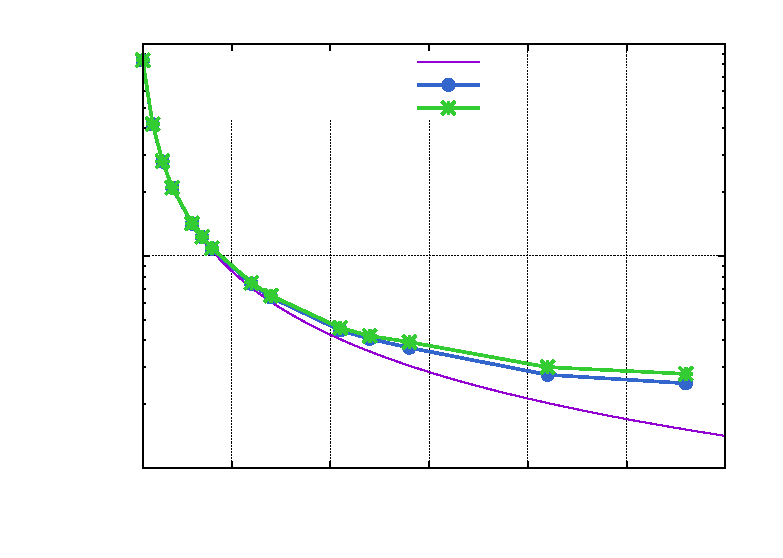
\includegraphics{plot-T-UDN-SM_nogatherInt_selected_500_selected_168_slide}}%
    \gplfronttext
  \end{picture}%
\endgroup
}
  \end{columns}
\end{frame}

\begin{frame}
  \frametitle{Confronto: tempo di servizio (3)}
  \begin{itemize}
  \item Tempo di interarrivo 4.627 \musec %57.831 \musec
  \item Dimensione delle matrici 280x280
  \end{itemize}
  \begin{columns}
    \column{.5\columnwidth}
    \resizebox{\columnwidth}{!}{% GNUPLOT: LaTeX picture with Postscript
\begingroup
  \makeatletter
  \providecommand\color[2][]{%
    \GenericError{(gnuplot) \space\space\space\@spaces}{%
      Package color not loaded in conjunction with
      terminal option `colourtext'%
    }{See the gnuplot documentation for explanation.%
    }{Either use 'blacktext' in gnuplot or load the package
      color.sty in LaTeX.}%
    \renewcommand\color[2][]{}%
  }%
  \providecommand\includegraphics[2][]{%
    \GenericError{(gnuplot) \space\space\space\@spaces}{%
      Package graphicx or graphics not loaded%
    }{See the gnuplot documentation for explanation.%
    }{The gnuplot epslatex terminal needs graphicx.sty or graphics.sty.}%
    \renewcommand\includegraphics[2][]{}%
  }%
  \providecommand\rotatebox[2]{#2}%
  \@ifundefined{ifGPcolor}{%
    \newif\ifGPcolor
    \GPcolortrue
  }{}%
  \@ifundefined{ifGPblacktext}{%
    \newif\ifGPblacktext
    \GPblacktexttrue
  }{}%
  % define a \g@addto@macro without @ in the name:
  \let\gplgaddtomacro\g@addto@macro
  % define empty templates for all commands taking text:
  \gdef\gplbacktext{}%
  \gdef\gplfronttext{}%
  \makeatother
  \ifGPblacktext
    % no textcolor at all
    \def\colorrgb#1{}%
    \def\colorgray#1{}%
  \else
    % gray or color?
    \ifGPcolor
      \def\colorrgb#1{\color[rgb]{#1}}%
      \def\colorgray#1{\color[gray]{#1}}%
      \expandafter\def\csname LTw\endcsname{\color{white}}%
      \expandafter\def\csname LTb\endcsname{\color{black}}%
      \expandafter\def\csname LTa\endcsname{\color{black}}%
      \expandafter\def\csname LT0\endcsname{\color[rgb]{1,0,0}}%
      \expandafter\def\csname LT1\endcsname{\color[rgb]{0,1,0}}%
      \expandafter\def\csname LT2\endcsname{\color[rgb]{0,0,1}}%
      \expandafter\def\csname LT3\endcsname{\color[rgb]{1,0,1}}%
      \expandafter\def\csname LT4\endcsname{\color[rgb]{0,1,1}}%
      \expandafter\def\csname LT5\endcsname{\color[rgb]{1,1,0}}%
      \expandafter\def\csname LT6\endcsname{\color[rgb]{0,0,0}}%
      \expandafter\def\csname LT7\endcsname{\color[rgb]{1,0.3,0}}%
      \expandafter\def\csname LT8\endcsname{\color[rgb]{0.5,0.5,0.5}}%
    \else
      % gray
      \def\colorrgb#1{\color{black}}%
      \def\colorgray#1{\color[gray]{#1}}%
      \expandafter\def\csname LTw\endcsname{\color{white}}%
      \expandafter\def\csname LTb\endcsname{\color{black}}%
      \expandafter\def\csname LTa\endcsname{\color{black}}%
      \expandafter\def\csname LT0\endcsname{\color{black}}%
      \expandafter\def\csname LT1\endcsname{\color{black}}%
      \expandafter\def\csname LT2\endcsname{\color{black}}%
      \expandafter\def\csname LT3\endcsname{\color{black}}%
      \expandafter\def\csname LT4\endcsname{\color{black}}%
      \expandafter\def\csname LT5\endcsname{\color{black}}%
      \expandafter\def\csname LT6\endcsname{\color{black}}%
      \expandafter\def\csname LT7\endcsname{\color{black}}%
      \expandafter\def\csname LT8\endcsname{\color{black}}%
    \fi
  \fi
  \setlength{\unitlength}{0.0500bp}%
  \begin{picture}(7200.00,5040.00)%
    \gplgaddtomacro\gplbacktext{%
      \csname LTb\endcsname%
      \put(814,1325){\makebox(0,0)[r]{\strut{} 10}}%
      \csname LTb\endcsname%
      \put(814,2015){\makebox(0,0)[r]{\strut{} 20}}%
      \csname LTb\endcsname%
      \put(814,2705){\makebox(0,0)[r]{\strut{} 30}}%
      \csname LTb\endcsname%
      \put(814,3395){\makebox(0,0)[r]{\strut{} 40}}%
      \csname LTb\endcsname%
      \put(814,4085){\makebox(0,0)[r]{\strut{} 50}}%
      \csname LTb\endcsname%
      \put(814,4775){\makebox(0,0)[r]{\strut{} 60}}%
      \csname LTb\endcsname%
      \put(1839,484){\makebox(0,0){\strut{} 10}}%
      \csname LTb\endcsname%
      \put(2832,484){\makebox(0,0){\strut{} 20}}%
      \csname LTb\endcsname%
      \put(3825,484){\makebox(0,0){\strut{} 30}}%
      \csname LTb\endcsname%
      \put(4818,484){\makebox(0,0){\strut{} 40}}%
      \csname LTb\endcsname%
      \put(5810,484){\makebox(0,0){\strut{} 50}}%
      \csname LTb\endcsname%
      \put(6803,484){\makebox(0,0){\strut{} 60}}%
      \put(176,2739){\rotatebox{-270}{\makebox(0,0){\strut{}scalability}}}%
      \put(3874,154){\makebox(0,0){\strut{}$n$ parallel degree}}%
    }%
    \gplgaddtomacro\gplfronttext{%
      \csname LTb\endcsname%
      \put(3322,4602){\makebox(0,0)[r]{\strut{}ideal scalability}}%
      \csname LTb\endcsname%
      \put(3322,4382){\makebox(0,0)[r]{\strut{}udn udn}}%
      \csname LTb\endcsname%
      \put(3322,4162){\makebox(0,0)[r]{\strut{}sm sm}}%
    }%
    \gplbacktext
    \put(0,0){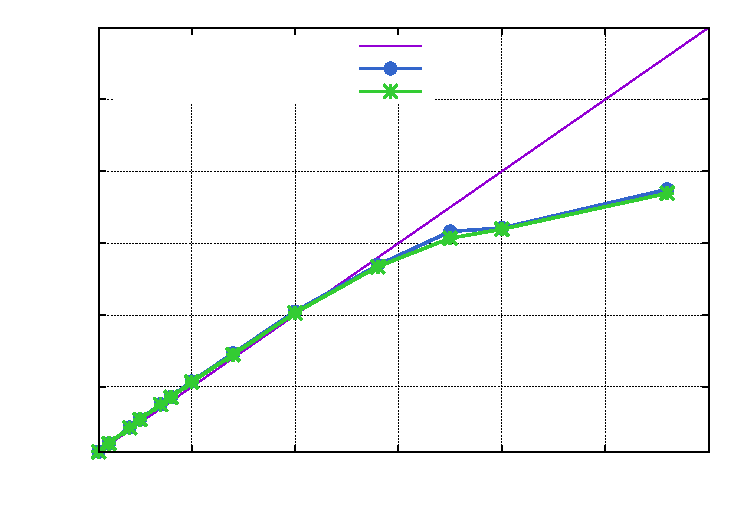
\includegraphics{plot-comp-T-s_nogatherInt_selected_500_50000_280_slide}}%
    \gplfronttext
  \end{picture}%
\endgroup
}
    \column{.5\columnwidth}
    \resizebox{\columnwidth}{!}{% GNUPLOT: LaTeX picture with Postscript
\begingroup
  \makeatletter
  \providecommand\color[2][]{%
    \GenericError{(gnuplot) \space\space\space\@spaces}{%
      Package color not loaded in conjunction with
      terminal option `colourtext'%
    }{See the gnuplot documentation for explanation.%
    }{Either use 'blacktext' in gnuplot or load the package
      color.sty in LaTeX.}%
    \renewcommand\color[2][]{}%
  }%
  \providecommand\includegraphics[2][]{%
    \GenericError{(gnuplot) \space\space\space\@spaces}{%
      Package graphicx or graphics not loaded%
    }{See the gnuplot documentation for explanation.%
    }{The gnuplot epslatex terminal needs graphicx.sty or graphics.sty.}%
    \renewcommand\includegraphics[2][]{}%
  }%
  \providecommand\rotatebox[2]{#2}%
  \@ifundefined{ifGPcolor}{%
    \newif\ifGPcolor
    \GPcolortrue
  }{}%
  \@ifundefined{ifGPblacktext}{%
    \newif\ifGPblacktext
    \GPblacktexttrue
  }{}%
  % define a \g@addto@macro without @ in the name:
  \let\gplgaddtomacro\g@addto@macro
  % define empty templates for all commands taking text:
  \gdef\gplbacktext{}%
  \gdef\gplfronttext{}%
  \makeatother
  \ifGPblacktext
    % no textcolor at all
    \def\colorrgb#1{}%
    \def\colorgray#1{}%
  \else
    % gray or color?
    \ifGPcolor
      \def\colorrgb#1{\color[rgb]{#1}}%
      \def\colorgray#1{\color[gray]{#1}}%
      \expandafter\def\csname LTw\endcsname{\color{white}}%
      \expandafter\def\csname LTb\endcsname{\color{black}}%
      \expandafter\def\csname LTa\endcsname{\color{black}}%
      \expandafter\def\csname LT0\endcsname{\color[rgb]{1,0,0}}%
      \expandafter\def\csname LT1\endcsname{\color[rgb]{0,1,0}}%
      \expandafter\def\csname LT2\endcsname{\color[rgb]{0,0,1}}%
      \expandafter\def\csname LT3\endcsname{\color[rgb]{1,0,1}}%
      \expandafter\def\csname LT4\endcsname{\color[rgb]{0,1,1}}%
      \expandafter\def\csname LT5\endcsname{\color[rgb]{1,1,0}}%
      \expandafter\def\csname LT6\endcsname{\color[rgb]{0,0,0}}%
      \expandafter\def\csname LT7\endcsname{\color[rgb]{1,0.3,0}}%
      \expandafter\def\csname LT8\endcsname{\color[rgb]{0.5,0.5,0.5}}%
    \else
      % gray
      \def\colorrgb#1{\color{black}}%
      \def\colorgray#1{\color[gray]{#1}}%
      \expandafter\def\csname LTw\endcsname{\color{white}}%
      \expandafter\def\csname LTb\endcsname{\color{black}}%
      \expandafter\def\csname LTa\endcsname{\color{black}}%
      \expandafter\def\csname LT0\endcsname{\color{black}}%
      \expandafter\def\csname LT1\endcsname{\color{black}}%
      \expandafter\def\csname LT2\endcsname{\color{black}}%
      \expandafter\def\csname LT3\endcsname{\color{black}}%
      \expandafter\def\csname LT4\endcsname{\color{black}}%
      \expandafter\def\csname LT5\endcsname{\color{black}}%
      \expandafter\def\csname LT6\endcsname{\color{black}}%
      \expandafter\def\csname LT7\endcsname{\color{black}}%
      \expandafter\def\csname LT8\endcsname{\color{black}}%
    \fi
  \fi
  \setlength{\unitlength}{0.0500bp}%
  \begin{picture}(7200.00,5040.00)%
    \gplgaddtomacro\gplbacktext{%
      \csname LTb\endcsname%
      \put(1210,704){\makebox(0,0)[r]{\strut{} 10}}%
      \csname LTb\endcsname%
      \put(1210,2061){\makebox(0,0)[r]{\strut{} 100}}%
      \csname LTb\endcsname%
      \put(1210,3418){\makebox(0,0)[r]{\strut{} 1000}}%
      \csname LTb\endcsname%
      \put(1210,4775){\makebox(0,0)[r]{\strut{} 10000}}%
      \csname LTb\endcsname%
      \put(2175,484){\makebox(0,0){\strut{} 10}}%
      \csname LTb\endcsname%
      \put(3101,484){\makebox(0,0){\strut{} 20}}%
      \csname LTb\endcsname%
      \put(4026,484){\makebox(0,0){\strut{} 30}}%
      \csname LTb\endcsname%
      \put(4952,484){\makebox(0,0){\strut{} 40}}%
      \csname LTb\endcsname%
      \put(5877,484){\makebox(0,0){\strut{} 50}}%
      \csname LTb\endcsname%
      \put(6803,484){\makebox(0,0){\strut{} 60}}%
      \put(176,2739){\rotatebox{-270}{\makebox(0,0){\strut{}service time ($\,\mu\mathrm{sec}$\,)}}}%
      \put(4072,154){\makebox(0,0){\strut{}$n$ parallel degree}}%
    }%
    \gplgaddtomacro\gplfronttext{%
      \csname LTb\endcsname%
      \put(3850,4602){\makebox(0,0)[r]{\strut{}ideal service time}}%
      \csname LTb\endcsname%
      \put(3850,4382){\makebox(0,0)[r]{\strut{}udn udn}}%
      \csname LTb\endcsname%
      \put(3850,4162){\makebox(0,0)[r]{\strut{}sm sm}}%
    }%
    \gplbacktext
    \put(0,0){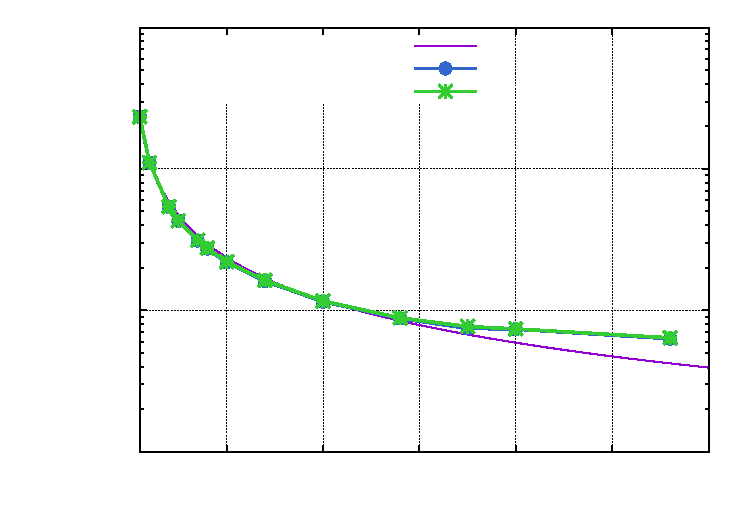
\includegraphics{plot-T-UDN-SM_nogatherInt_selected_500_selected_280_slide}}%
    \gplfronttext
  \end{picture}%
\endgroup
}
  \end{columns}
\end{frame}

\begin{frame}
  \frametitle{Confronto: tempo di servizio Multicast}
  \begin{columns}
    \column{.5\columnwidth}
    Dimensione delle matrici 56x56
    \column{.5\columnwidth}
    Dimensione delle matrici 280x280
  \end{columns}
  \vspace{5mm}
  \begin{columns}[c]
    \column{.5\columnwidth}
    \resizebox{\columnwidth}{!}{% GNUPLOT: LaTeX picture with Postscript
\begingroup
  \makeatletter
  \providecommand\color[2][]{%
    \GenericError{(gnuplot) \space\space\space\@spaces}{%
      Package color not loaded in conjunction with
      terminal option `colourtext'%
    }{See the gnuplot documentation for explanation.%
    }{Either use 'blacktext' in gnuplot or load the package
      color.sty in LaTeX.}%
    \renewcommand\color[2][]{}%
  }%
  \providecommand\includegraphics[2][]{%
    \GenericError{(gnuplot) \space\space\space\@spaces}{%
      Package graphicx or graphics not loaded%
    }{See the gnuplot documentation for explanation.%
    }{The gnuplot epslatex terminal needs graphicx.sty or graphics.sty.}%
    \renewcommand\includegraphics[2][]{}%
  }%
  \providecommand\rotatebox[2]{#2}%
  \@ifundefined{ifGPcolor}{%
    \newif\ifGPcolor
    \GPcolortrue
  }{}%
  \@ifundefined{ifGPblacktext}{%
    \newif\ifGPblacktext
    \GPblacktexttrue
  }{}%
  % define a \g@addto@macro without @ in the name:
  \let\gplgaddtomacro\g@addto@macro
  % define empty templates for all commands taking text:
  \gdef\gplbacktext{}%
  \gdef\gplfronttext{}%
  \makeatother
  \ifGPblacktext
    % no textcolor at all
    \def\colorrgb#1{}%
    \def\colorgray#1{}%
  \else
    % gray or color?
    \ifGPcolor
      \def\colorrgb#1{\color[rgb]{#1}}%
      \def\colorgray#1{\color[gray]{#1}}%
      \expandafter\def\csname LTw\endcsname{\color{white}}%
      \expandafter\def\csname LTb\endcsname{\color{black}}%
      \expandafter\def\csname LTa\endcsname{\color{black}}%
      \expandafter\def\csname LT0\endcsname{\color[rgb]{1,0,0}}%
      \expandafter\def\csname LT1\endcsname{\color[rgb]{0,1,0}}%
      \expandafter\def\csname LT2\endcsname{\color[rgb]{0,0,1}}%
      \expandafter\def\csname LT3\endcsname{\color[rgb]{1,0,1}}%
      \expandafter\def\csname LT4\endcsname{\color[rgb]{0,1,1}}%
      \expandafter\def\csname LT5\endcsname{\color[rgb]{1,1,0}}%
      \expandafter\def\csname LT6\endcsname{\color[rgb]{0,0,0}}%
      \expandafter\def\csname LT7\endcsname{\color[rgb]{1,0.3,0}}%
      \expandafter\def\csname LT8\endcsname{\color[rgb]{0.5,0.5,0.5}}%
    \else
      % gray
      \def\colorrgb#1{\color{black}}%
      \def\colorgray#1{\color[gray]{#1}}%
      \expandafter\def\csname LTw\endcsname{\color{white}}%
      \expandafter\def\csname LTb\endcsname{\color{black}}%
      \expandafter\def\csname LTa\endcsname{\color{black}}%
      \expandafter\def\csname LT0\endcsname{\color{black}}%
      \expandafter\def\csname LT1\endcsname{\color{black}}%
      \expandafter\def\csname LT2\endcsname{\color{black}}%
      \expandafter\def\csname LT3\endcsname{\color{black}}%
      \expandafter\def\csname LT4\endcsname{\color{black}}%
      \expandafter\def\csname LT5\endcsname{\color{black}}%
      \expandafter\def\csname LT6\endcsname{\color{black}}%
      \expandafter\def\csname LT7\endcsname{\color{black}}%
      \expandafter\def\csname LT8\endcsname{\color{black}}%
    \fi
  \fi
  \setlength{\unitlength}{0.0500bp}%
  \begin{picture}(7200.00,5040.00)%
    \gplgaddtomacro\gplbacktext{%
      \csname LTb\endcsname%
      \put(946,704){\makebox(0,0)[r]{\strut{} 0}}%
      \csname LTb\endcsname%
      \put(946,1629){\makebox(0,0)[r]{\strut{} 0.5}}%
      \csname LTb\endcsname%
      \put(946,2554){\makebox(0,0)[r]{\strut{} 1}}%
      \csname LTb\endcsname%
      \put(946,3480){\makebox(0,0)[r]{\strut{} 1.5}}%
      \csname LTb\endcsname%
      \put(946,4405){\makebox(0,0)[r]{\strut{} 2}}%
      \csname LTb\endcsname%
      \put(1951,484){\makebox(0,0){\strut{} 10}}%
      \csname LTb\endcsname%
      \put(2922,484){\makebox(0,0){\strut{} 20}}%
      \csname LTb\endcsname%
      \put(3892,484){\makebox(0,0){\strut{} 30}}%
      \csname LTb\endcsname%
      \put(4862,484){\makebox(0,0){\strut{} 40}}%
      \csname LTb\endcsname%
      \put(5833,484){\makebox(0,0){\strut{} 50}}%
      \csname LTb\endcsname%
      \put(6803,484){\makebox(0,0){\strut{} 60}}%
      \put(176,2739){\rotatebox{-270}{\makebox(0,0){\strut{}multicast service time $(\,\mu\textrm{sec}\,)$}}}%
      \put(3940,154){\makebox(0,0){\strut{}$n$ parallel degree}}%
    }%
    \gplgaddtomacro\gplfronttext{%
      \csname LTb\endcsname%
      \put(2134,4602){\makebox(0,0)[r]{\strut{}udn udn}}%
      \csname LTb\endcsname%
      \put(2134,4382){\makebox(0,0)[r]{\strut{}sm sm}}%
    }%
    \gplbacktext
    \put(0,0){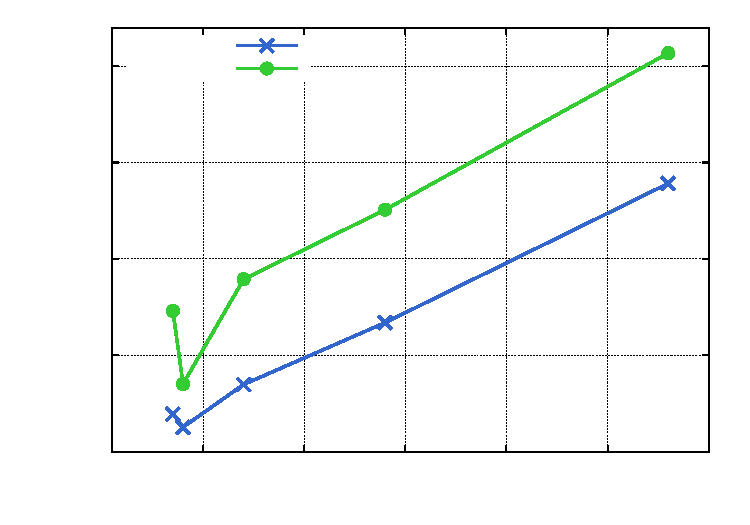
\includegraphics{plot-Tmult-UDN-SM-millis_nogatherInt_selected_500_selected_56_slide}}%
    \gplfronttext
  \end{picture}%
\endgroup
}
    \column{.5\columnwidth}
    \resizebox{\columnwidth}{!}{% GNUPLOT: LaTeX picture with Postscript
\begingroup
  \makeatletter
  \providecommand\color[2][]{%
    \GenericError{(gnuplot) \space\space\space\@spaces}{%
      Package color not loaded in conjunction with
      terminal option `colourtext'%
    }{See the gnuplot documentation for explanation.%
    }{Either use 'blacktext' in gnuplot or load the package
      color.sty in LaTeX.}%
    \renewcommand\color[2][]{}%
  }%
  \providecommand\includegraphics[2][]{%
    \GenericError{(gnuplot) \space\space\space\@spaces}{%
      Package graphicx or graphics not loaded%
    }{See the gnuplot documentation for explanation.%
    }{The gnuplot epslatex terminal needs graphicx.sty or graphics.sty.}%
    \renewcommand\includegraphics[2][]{}%
  }%
  \providecommand\rotatebox[2]{#2}%
  \@ifundefined{ifGPcolor}{%
    \newif\ifGPcolor
    \GPcolortrue
  }{}%
  \@ifundefined{ifGPblacktext}{%
    \newif\ifGPblacktext
    \GPblacktexttrue
  }{}%
  % define a \g@addto@macro without @ in the name:
  \let\gplgaddtomacro\g@addto@macro
  % define empty templates for all commands taking text:
  \gdef\gplbacktext{}%
  \gdef\gplfronttext{}%
  \makeatother
  \ifGPblacktext
    % no textcolor at all
    \def\colorrgb#1{}%
    \def\colorgray#1{}%
  \else
    % gray or color?
    \ifGPcolor
      \def\colorrgb#1{\color[rgb]{#1}}%
      \def\colorgray#1{\color[gray]{#1}}%
      \expandafter\def\csname LTw\endcsname{\color{white}}%
      \expandafter\def\csname LTb\endcsname{\color{black}}%
      \expandafter\def\csname LTa\endcsname{\color{black}}%
      \expandafter\def\csname LT0\endcsname{\color[rgb]{1,0,0}}%
      \expandafter\def\csname LT1\endcsname{\color[rgb]{0,1,0}}%
      \expandafter\def\csname LT2\endcsname{\color[rgb]{0,0,1}}%
      \expandafter\def\csname LT3\endcsname{\color[rgb]{1,0,1}}%
      \expandafter\def\csname LT4\endcsname{\color[rgb]{0,1,1}}%
      \expandafter\def\csname LT5\endcsname{\color[rgb]{1,1,0}}%
      \expandafter\def\csname LT6\endcsname{\color[rgb]{0,0,0}}%
      \expandafter\def\csname LT7\endcsname{\color[rgb]{1,0.3,0}}%
      \expandafter\def\csname LT8\endcsname{\color[rgb]{0.5,0.5,0.5}}%
    \else
      % gray
      \def\colorrgb#1{\color{black}}%
      \def\colorgray#1{\color[gray]{#1}}%
      \expandafter\def\csname LTw\endcsname{\color{white}}%
      \expandafter\def\csname LTb\endcsname{\color{black}}%
      \expandafter\def\csname LTa\endcsname{\color{black}}%
      \expandafter\def\csname LT0\endcsname{\color{black}}%
      \expandafter\def\csname LT1\endcsname{\color{black}}%
      \expandafter\def\csname LT2\endcsname{\color{black}}%
      \expandafter\def\csname LT3\endcsname{\color{black}}%
      \expandafter\def\csname LT4\endcsname{\color{black}}%
      \expandafter\def\csname LT5\endcsname{\color{black}}%
      \expandafter\def\csname LT6\endcsname{\color{black}}%
      \expandafter\def\csname LT7\endcsname{\color{black}}%
      \expandafter\def\csname LT8\endcsname{\color{black}}%
    \fi
  \fi
  \setlength{\unitlength}{0.0500bp}%
  \begin{picture}(7200.00,5040.00)%
    \gplgaddtomacro\gplbacktext{%
      \csname LTb\endcsname%
      \put(946,704){\makebox(0,0)[r]{\strut{} 0}}%
      \csname LTb\endcsname%
      \put(946,1629){\makebox(0,0)[r]{\strut{} 0.5}}%
      \csname LTb\endcsname%
      \put(946,2554){\makebox(0,0)[r]{\strut{} 1}}%
      \csname LTb\endcsname%
      \put(946,3480){\makebox(0,0)[r]{\strut{} 1.5}}%
      \csname LTb\endcsname%
      \put(946,4405){\makebox(0,0)[r]{\strut{} 2}}%
      \csname LTb\endcsname%
      \put(1951,484){\makebox(0,0){\strut{} 10}}%
      \csname LTb\endcsname%
      \put(2922,484){\makebox(0,0){\strut{} 20}}%
      \csname LTb\endcsname%
      \put(3892,484){\makebox(0,0){\strut{} 30}}%
      \csname LTb\endcsname%
      \put(4862,484){\makebox(0,0){\strut{} 40}}%
      \csname LTb\endcsname%
      \put(5833,484){\makebox(0,0){\strut{} 50}}%
      \csname LTb\endcsname%
      \put(6803,484){\makebox(0,0){\strut{} 60}}%
      \put(176,2739){\rotatebox{-270}{\makebox(0,0){\strut{}multicast service time $(\,\mu\textrm{sec}\,)$}}}%
      \put(3940,154){\makebox(0,0){\strut{}$n$ parallel degree}}%
    }%
    \gplgaddtomacro\gplfronttext{%
      \csname LTb\endcsname%
      \put(2134,4602){\makebox(0,0)[r]{\strut{}udn udn}}%
      \csname LTb\endcsname%
      \put(2134,4382){\makebox(0,0)[r]{\strut{}sm sm}}%
    }%
    \gplbacktext
    \put(0,0){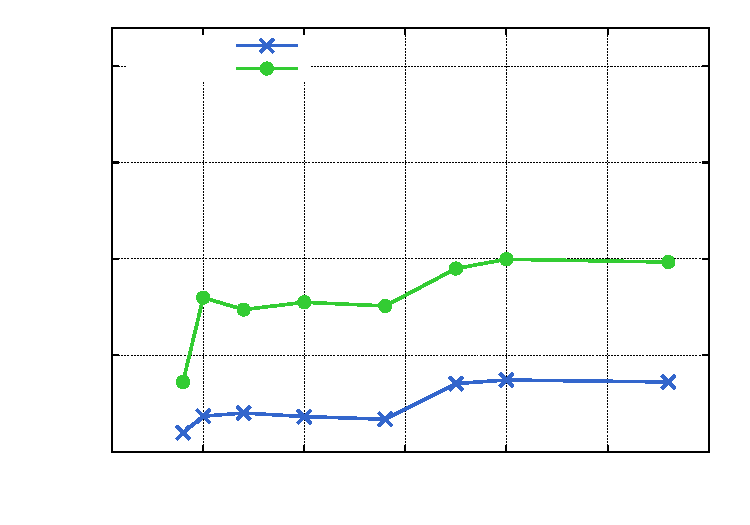
\includegraphics{plot-Tmult-UDN-SM-millis_nogatherInt_selected_500_selected_280_slide}}%
    \gplfronttext
  \end{picture}%
\endgroup
}
  \end{columns}  
\end{frame}

\begin{frame}
  \frametitle{Confronto: tempo di calcolo di un singolo prodotto scalare}
  \begin{columns}[c]
    \column{.5\columnwidth}
    \resizebox{\columnwidth}{!}{% GNUPLOT: LaTeX picture with Postscript
\begingroup
  \makeatletter
  \providecommand\color[2][]{%
    \GenericError{(gnuplot) \space\space\space\@spaces}{%
      Package color not loaded in conjunction with
      terminal option `colourtext'%
    }{See the gnuplot documentation for explanation.%
    }{Either use 'blacktext' in gnuplot or load the package
      color.sty in LaTeX.}%
    \renewcommand\color[2][]{}%
  }%
  \providecommand\includegraphics[2][]{%
    \GenericError{(gnuplot) \space\space\space\@spaces}{%
      Package graphicx or graphics not loaded%
    }{See the gnuplot documentation for explanation.%
    }{The gnuplot epslatex terminal needs graphicx.sty or graphics.sty.}%
    \renewcommand\includegraphics[2][]{}%
  }%
  \providecommand\rotatebox[2]{#2}%
  \@ifundefined{ifGPcolor}{%
    \newif\ifGPcolor
    \GPcolortrue
  }{}%
  \@ifundefined{ifGPblacktext}{%
    \newif\ifGPblacktext
    \GPblacktextfalse
  }{}%
  % define a \g@addto@macro without @ in the name:
  \let\gplgaddtomacro\g@addto@macro
  % define empty templates for all commands taking text:
  \gdef\gplbacktext{}%
  \gdef\gplfronttext{}%
  \makeatother
  \ifGPblacktext
    % no textcolor at all
    \def\colorrgb#1{}%
    \def\colorgray#1{}%
  \else
    % gray or color?
    \ifGPcolor
      \def\colorrgb#1{\color[rgb]{#1}}%
      \def\colorgray#1{\color[gray]{#1}}%
      \expandafter\def\csname LTw\endcsname{\color{white}}%
      \expandafter\def\csname LTb\endcsname{\color{black}}%
      \expandafter\def\csname LTa\endcsname{\color{black}}%
      \expandafter\def\csname LT0\endcsname{\color[rgb]{1,0,0}}%
      \expandafter\def\csname LT1\endcsname{\color[rgb]{0,1,0}}%
      \expandafter\def\csname LT2\endcsname{\color[rgb]{0,0,1}}%
      \expandafter\def\csname LT3\endcsname{\color[rgb]{1,0,1}}%
      \expandafter\def\csname LT4\endcsname{\color[rgb]{0,1,1}}%
      \expandafter\def\csname LT5\endcsname{\color[rgb]{1,1,0}}%
      \expandafter\def\csname LT6\endcsname{\color[rgb]{0,0,0}}%
      \expandafter\def\csname LT7\endcsname{\color[rgb]{1,0.3,0}}%
      \expandafter\def\csname LT8\endcsname{\color[rgb]{0.5,0.5,0.5}}%
    \else
      % gray
      \def\colorrgb#1{\color{black}}%
      \def\colorgray#1{\color[gray]{#1}}%
      \expandafter\def\csname LTw\endcsname{\color{white}}%
      \expandafter\def\csname LTb\endcsname{\color{black}}%
      \expandafter\def\csname LTa\endcsname{\color{black}}%
      \expandafter\def\csname LT0\endcsname{\color{black}}%
      \expandafter\def\csname LT1\endcsname{\color{black}}%
      \expandafter\def\csname LT2\endcsname{\color{black}}%
      \expandafter\def\csname LT3\endcsname{\color{black}}%
      \expandafter\def\csname LT4\endcsname{\color{black}}%
      \expandafter\def\csname LT5\endcsname{\color{black}}%
      \expandafter\def\csname LT6\endcsname{\color{black}}%
      \expandafter\def\csname LT7\endcsname{\color{black}}%
      \expandafter\def\csname LT8\endcsname{\color{black}}%
    \fi
  \fi
  \setlength{\unitlength}{0.0500bp}%
  \begin{picture}(7200.00,5040.00)%
    \gplgaddtomacro\gplbacktext{%
      \csname LTb\endcsname%
      \put(946,1074){\makebox(0,0)[r]{\strut{} 1}}%
      \csname LTb\endcsname%
      \put(946,1999){\makebox(0,0)[r]{\strut{} 1.5}}%
      \csname LTb\endcsname%
      \put(946,2925){\makebox(0,0)[r]{\strut{} 2}}%
      \csname LTb\endcsname%
      \put(946,3850){\makebox(0,0)[r]{\strut{} 2.5}}%
      \csname LTb\endcsname%
      \put(946,4775){\makebox(0,0)[r]{\strut{} 3}}%
      \csname LTb\endcsname%
      \put(1951,484){\makebox(0,0){\strut{} 10}}%
      \csname LTb\endcsname%
      \put(2922,484){\makebox(0,0){\strut{} 20}}%
      \csname LTb\endcsname%
      \put(3892,484){\makebox(0,0){\strut{} 30}}%
      \csname LTb\endcsname%
      \put(4862,484){\makebox(0,0){\strut{} 40}}%
      \csname LTb\endcsname%
      \put(5833,484){\makebox(0,0){\strut{} 50}}%
      \csname LTb\endcsname%
      \put(6803,484){\makebox(0,0){\strut{} 60}}%
      \put(176,2739){\rotatebox{-270}{\makebox(0,0){\strut{}$T_{\textrm{row}}^{\phantom{row}(n)} / T_{\textrm{row}}^{\phantom{row}(1)}$}}}%
      \put(3940,154){\makebox(0,0){\strut{}$n$ parallel degree}}%
    }%
    \gplgaddtomacro\gplfronttext{%
      \csname LTb\endcsname%
      \put(3718,4602){\makebox(0,0)[r]{\strut{}Matrix Size 280x280}}%
      \csname LTb\endcsname%
      \put(3718,4382){\makebox(0,0)[r]{\strut{}Matrix Size 168x168}}%
      \csname LTb\endcsname%
      \put(3718,4162){\makebox(0,0)[r]{\strut{}Matrix Size 56x56}}%
    }%
    \gplbacktext
    \put(0,0){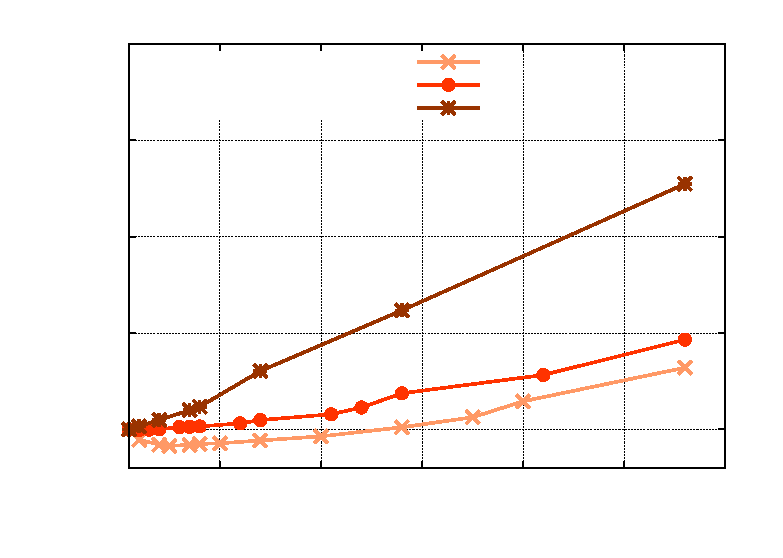
\includegraphics{plot-rowCalcT_nogatherInt_00_500_4000_all_slide}}%
    \gplfronttext
  \end{picture}%
\endgroup
}
    \column{.5\columnwidth}
    \resizebox{\columnwidth}{!}{% GNUPLOT: LaTeX picture with Postscript
\begingroup
  \makeatletter
  \providecommand\color[2][]{%
    \GenericError{(gnuplot) \space\space\space\@spaces}{%
      Package color not loaded in conjunction with
      terminal option `colourtext'%
    }{See the gnuplot documentation for explanation.%
    }{Either use 'blacktext' in gnuplot or load the package
      color.sty in LaTeX.}%
    \renewcommand\color[2][]{}%
  }%
  \providecommand\includegraphics[2][]{%
    \GenericError{(gnuplot) \space\space\space\@spaces}{%
      Package graphicx or graphics not loaded%
    }{See the gnuplot documentation for explanation.%
    }{The gnuplot epslatex terminal needs graphicx.sty or graphics.sty.}%
    \renewcommand\includegraphics[2][]{}%
  }%
  \providecommand\rotatebox[2]{#2}%
  \@ifundefined{ifGPcolor}{%
    \newif\ifGPcolor
    \GPcolortrue
  }{}%
  \@ifundefined{ifGPblacktext}{%
    \newif\ifGPblacktext
    \GPblacktextfalse
  }{}%
  % define a \g@addto@macro without @ in the name:
  \let\gplgaddtomacro\g@addto@macro
  % define empty templates for all commands taking text:
  \gdef\gplbacktext{}%
  \gdef\gplfronttext{}%
  \makeatother
  \ifGPblacktext
    % no textcolor at all
    \def\colorrgb#1{}%
    \def\colorgray#1{}%
  \else
    % gray or color?
    \ifGPcolor
      \def\colorrgb#1{\color[rgb]{#1}}%
      \def\colorgray#1{\color[gray]{#1}}%
      \expandafter\def\csname LTw\endcsname{\color{white}}%
      \expandafter\def\csname LTb\endcsname{\color{black}}%
      \expandafter\def\csname LTa\endcsname{\color{black}}%
      \expandafter\def\csname LT0\endcsname{\color[rgb]{1,0,0}}%
      \expandafter\def\csname LT1\endcsname{\color[rgb]{0,1,0}}%
      \expandafter\def\csname LT2\endcsname{\color[rgb]{0,0,1}}%
      \expandafter\def\csname LT3\endcsname{\color[rgb]{1,0,1}}%
      \expandafter\def\csname LT4\endcsname{\color[rgb]{0,1,1}}%
      \expandafter\def\csname LT5\endcsname{\color[rgb]{1,1,0}}%
      \expandafter\def\csname LT6\endcsname{\color[rgb]{0,0,0}}%
      \expandafter\def\csname LT7\endcsname{\color[rgb]{1,0.3,0}}%
      \expandafter\def\csname LT8\endcsname{\color[rgb]{0.5,0.5,0.5}}%
    \else
      % gray
      \def\colorrgb#1{\color{black}}%
      \def\colorgray#1{\color[gray]{#1}}%
      \expandafter\def\csname LTw\endcsname{\color{white}}%
      \expandafter\def\csname LTb\endcsname{\color{black}}%
      \expandafter\def\csname LTa\endcsname{\color{black}}%
      \expandafter\def\csname LT0\endcsname{\color{black}}%
      \expandafter\def\csname LT1\endcsname{\color{black}}%
      \expandafter\def\csname LT2\endcsname{\color{black}}%
      \expandafter\def\csname LT3\endcsname{\color{black}}%
      \expandafter\def\csname LT4\endcsname{\color{black}}%
      \expandafter\def\csname LT5\endcsname{\color{black}}%
      \expandafter\def\csname LT6\endcsname{\color{black}}%
      \expandafter\def\csname LT7\endcsname{\color{black}}%
      \expandafter\def\csname LT8\endcsname{\color{black}}%
    \fi
  \fi
  \setlength{\unitlength}{0.0500bp}%
  \begin{picture}(7200.00,5040.00)%
    \gplgaddtomacro\gplbacktext{%
      \csname LTb\endcsname%
      \put(946,1074){\makebox(0,0)[r]{\strut{} 1}}%
      \csname LTb\endcsname%
      \put(946,1999){\makebox(0,0)[r]{\strut{} 1.5}}%
      \csname LTb\endcsname%
      \put(946,2925){\makebox(0,0)[r]{\strut{} 2}}%
      \csname LTb\endcsname%
      \put(946,3850){\makebox(0,0)[r]{\strut{} 2.5}}%
      \csname LTb\endcsname%
      \put(946,4775){\makebox(0,0)[r]{\strut{} 3}}%
      \csname LTb\endcsname%
      \put(1951,484){\makebox(0,0){\strut{} 10}}%
      \csname LTb\endcsname%
      \put(2922,484){\makebox(0,0){\strut{} 20}}%
      \csname LTb\endcsname%
      \put(3892,484){\makebox(0,0){\strut{} 30}}%
      \csname LTb\endcsname%
      \put(4862,484){\makebox(0,0){\strut{} 40}}%
      \csname LTb\endcsname%
      \put(5833,484){\makebox(0,0){\strut{} 50}}%
      \csname LTb\endcsname%
      \put(6803,484){\makebox(0,0){\strut{} 60}}%
      \put(176,2739){\rotatebox{-270}{\makebox(0,0){\strut{}$T_{\textrm{row}}^{\phantom{row}(n)} / T_{\textrm{row}}^{\phantom{row}(1)}$}}}%
      \put(3940,154){\makebox(0,0){\strut{}$n$ parallel degree}}%
    }%
    \gplgaddtomacro\gplfronttext{%
      \csname LTb\endcsname%
      \put(3718,4602){\makebox(0,0)[r]{\strut{}Matrix Size 280x280}}%
      \csname LTb\endcsname%
      \put(3718,4382){\makebox(0,0)[r]{\strut{}Matrix Size 168x168}}%
      \csname LTb\endcsname%
      \put(3718,4162){\makebox(0,0)[r]{\strut{}Matrix Size 56x56}}%
    }%
    \gplbacktext
    \put(0,0){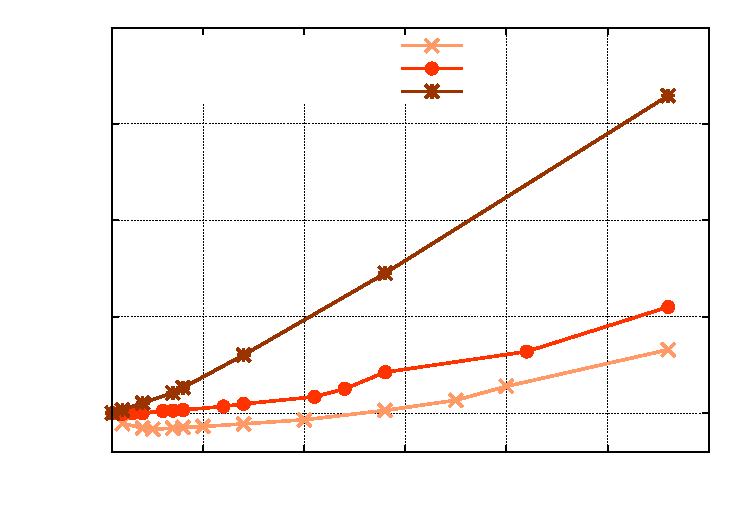
\includegraphics{plot-rowCalcT_nogatherInt_11_500_4000_all_slide}}%
    \gplfronttext
  \end{picture}%
\endgroup
}
  \end{columns} 
\end{frame}

\begin{frame}
  \frametitle{Confronto: tempo di calcolo di un singolo prodotto scalare}
  \begin{columns}[c]
    \column{.5\columnwidth}
    \resizebox{\columnwidth}{!}{% GNUPLOT: LaTeX picture with Postscript
\begingroup
  \makeatletter
  \providecommand\color[2][]{%
    \GenericError{(gnuplot) \space\space\space\@spaces}{%
      Package color not loaded in conjunction with
      terminal option `colourtext'%
    }{See the gnuplot documentation for explanation.%
    }{Either use 'blacktext' in gnuplot or load the package
      color.sty in LaTeX.}%
    \renewcommand\color[2][]{}%
  }%
  \providecommand\includegraphics[2][]{%
    \GenericError{(gnuplot) \space\space\space\@spaces}{%
      Package graphicx or graphics not loaded%
    }{See the gnuplot documentation for explanation.%
    }{The gnuplot epslatex terminal needs graphicx.sty or graphics.sty.}%
    \renewcommand\includegraphics[2][]{}%
  }%
  \providecommand\rotatebox[2]{#2}%
  \@ifundefined{ifGPcolor}{%
    \newif\ifGPcolor
    \GPcolortrue
  }{}%
  \@ifundefined{ifGPblacktext}{%
    \newif\ifGPblacktext
    \GPblacktextfalse
  }{}%
  % define a \g@addto@macro without @ in the name:
  \let\gplgaddtomacro\g@addto@macro
  % define empty templates for all commands taking text:
  \gdef\gplbacktext{}%
  \gdef\gplfronttext{}%
  \makeatother
  \ifGPblacktext
    % no textcolor at all
    \def\colorrgb#1{}%
    \def\colorgray#1{}%
  \else
    % gray or color?
    \ifGPcolor
      \def\colorrgb#1{\color[rgb]{#1}}%
      \def\colorgray#1{\color[gray]{#1}}%
      \expandafter\def\csname LTw\endcsname{\color{white}}%
      \expandafter\def\csname LTb\endcsname{\color{black}}%
      \expandafter\def\csname LTa\endcsname{\color{black}}%
      \expandafter\def\csname LT0\endcsname{\color[rgb]{1,0,0}}%
      \expandafter\def\csname LT1\endcsname{\color[rgb]{0,1,0}}%
      \expandafter\def\csname LT2\endcsname{\color[rgb]{0,0,1}}%
      \expandafter\def\csname LT3\endcsname{\color[rgb]{1,0,1}}%
      \expandafter\def\csname LT4\endcsname{\color[rgb]{0,1,1}}%
      \expandafter\def\csname LT5\endcsname{\color[rgb]{1,1,0}}%
      \expandafter\def\csname LT6\endcsname{\color[rgb]{0,0,0}}%
      \expandafter\def\csname LT7\endcsname{\color[rgb]{1,0.3,0}}%
      \expandafter\def\csname LT8\endcsname{\color[rgb]{0.5,0.5,0.5}}%
    \else
      % gray
      \def\colorrgb#1{\color{black}}%
      \def\colorgray#1{\color[gray]{#1}}%
      \expandafter\def\csname LTw\endcsname{\color{white}}%
      \expandafter\def\csname LTb\endcsname{\color{black}}%
      \expandafter\def\csname LTa\endcsname{\color{black}}%
      \expandafter\def\csname LT0\endcsname{\color{black}}%
      \expandafter\def\csname LT1\endcsname{\color{black}}%
      \expandafter\def\csname LT2\endcsname{\color{black}}%
      \expandafter\def\csname LT3\endcsname{\color{black}}%
      \expandafter\def\csname LT4\endcsname{\color{black}}%
      \expandafter\def\csname LT5\endcsname{\color{black}}%
      \expandafter\def\csname LT6\endcsname{\color{black}}%
      \expandafter\def\csname LT7\endcsname{\color{black}}%
      \expandafter\def\csname LT8\endcsname{\color{black}}%
    \fi
  \fi
  \setlength{\unitlength}{0.0500bp}%
  \begin{picture}(7200.00,5040.00)%
    \gplgaddtomacro\gplbacktext{%
      \csname LTb\endcsname%
      \put(946,1074){\makebox(0,0)[r]{\strut{} 1}}%
      \csname LTb\endcsname%
      \put(946,1999){\makebox(0,0)[r]{\strut{} 1.5}}%
      \csname LTb\endcsname%
      \put(946,2925){\makebox(0,0)[r]{\strut{} 2}}%
      \csname LTb\endcsname%
      \put(946,3850){\makebox(0,0)[r]{\strut{} 2.5}}%
      \csname LTb\endcsname%
      \put(946,4775){\makebox(0,0)[r]{\strut{} 3}}%
      \csname LTb\endcsname%
      \put(1951,484){\makebox(0,0){\strut{} 10}}%
      \csname LTb\endcsname%
      \put(2922,484){\makebox(0,0){\strut{} 20}}%
      \csname LTb\endcsname%
      \put(3892,484){\makebox(0,0){\strut{} 30}}%
      \csname LTb\endcsname%
      \put(4862,484){\makebox(0,0){\strut{} 40}}%
      \csname LTb\endcsname%
      \put(5833,484){\makebox(0,0){\strut{} 50}}%
      \csname LTb\endcsname%
      \put(6803,484){\makebox(0,0){\strut{} 60}}%
      \put(176,2739){\rotatebox{-270}{\makebox(0,0){\strut{}$T_{\textrm{row}}^{\phantom{row}(n)} / T_{\textrm{row}}^{\phantom{row}(1)}$}}}%
      \put(3940,154){\makebox(0,0){\strut{}$n$ parallel degree}}%
    }%
    \gplgaddtomacro\gplfronttext{%
      \csname LTb\endcsname%
      \put(3718,4602){\makebox(0,0)[r]{\strut{}Matrix Size 280x280}}%
      \csname LTb\endcsname%
      \put(3718,4382){\makebox(0,0)[r]{\strut{}Matrix Size 168x168}}%
      \csname LTb\endcsname%
      \put(3718,4162){\makebox(0,0)[r]{\strut{}Matrix Size 56x56}}%
    }%
    \gplbacktext
    \put(0,0){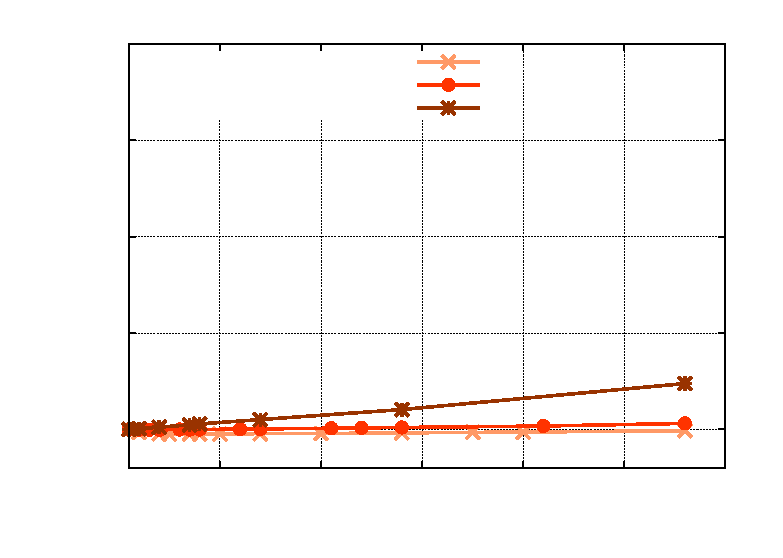
\includegraphics{plot-rowCalcT_nogatherFloat_00_500_4000_all_slide}}%
    \gplfronttext
  \end{picture}%
\endgroup
}
    \column{.5\columnwidth}
    \resizebox{\columnwidth}{!}{% GNUPLOT: LaTeX picture with Postscript
\begingroup
  \makeatletter
  \providecommand\color[2][]{%
    \GenericError{(gnuplot) \space\space\space\@spaces}{%
      Package color not loaded in conjunction with
      terminal option `colourtext'%
    }{See the gnuplot documentation for explanation.%
    }{Either use 'blacktext' in gnuplot or load the package
      color.sty in LaTeX.}%
    \renewcommand\color[2][]{}%
  }%
  \providecommand\includegraphics[2][]{%
    \GenericError{(gnuplot) \space\space\space\@spaces}{%
      Package graphicx or graphics not loaded%
    }{See the gnuplot documentation for explanation.%
    }{The gnuplot epslatex terminal needs graphicx.sty or graphics.sty.}%
    \renewcommand\includegraphics[2][]{}%
  }%
  \providecommand\rotatebox[2]{#2}%
  \@ifundefined{ifGPcolor}{%
    \newif\ifGPcolor
    \GPcolortrue
  }{}%
  \@ifundefined{ifGPblacktext}{%
    \newif\ifGPblacktext
    \GPblacktextfalse
  }{}%
  % define a \g@addto@macro without @ in the name:
  \let\gplgaddtomacro\g@addto@macro
  % define empty templates for all commands taking text:
  \gdef\gplbacktext{}%
  \gdef\gplfronttext{}%
  \makeatother
  \ifGPblacktext
    % no textcolor at all
    \def\colorrgb#1{}%
    \def\colorgray#1{}%
  \else
    % gray or color?
    \ifGPcolor
      \def\colorrgb#1{\color[rgb]{#1}}%
      \def\colorgray#1{\color[gray]{#1}}%
      \expandafter\def\csname LTw\endcsname{\color{white}}%
      \expandafter\def\csname LTb\endcsname{\color{black}}%
      \expandafter\def\csname LTa\endcsname{\color{black}}%
      \expandafter\def\csname LT0\endcsname{\color[rgb]{1,0,0}}%
      \expandafter\def\csname LT1\endcsname{\color[rgb]{0,1,0}}%
      \expandafter\def\csname LT2\endcsname{\color[rgb]{0,0,1}}%
      \expandafter\def\csname LT3\endcsname{\color[rgb]{1,0,1}}%
      \expandafter\def\csname LT4\endcsname{\color[rgb]{0,1,1}}%
      \expandafter\def\csname LT5\endcsname{\color[rgb]{1,1,0}}%
      \expandafter\def\csname LT6\endcsname{\color[rgb]{0,0,0}}%
      \expandafter\def\csname LT7\endcsname{\color[rgb]{1,0.3,0}}%
      \expandafter\def\csname LT8\endcsname{\color[rgb]{0.5,0.5,0.5}}%
    \else
      % gray
      \def\colorrgb#1{\color{black}}%
      \def\colorgray#1{\color[gray]{#1}}%
      \expandafter\def\csname LTw\endcsname{\color{white}}%
      \expandafter\def\csname LTb\endcsname{\color{black}}%
      \expandafter\def\csname LTa\endcsname{\color{black}}%
      \expandafter\def\csname LT0\endcsname{\color{black}}%
      \expandafter\def\csname LT1\endcsname{\color{black}}%
      \expandafter\def\csname LT2\endcsname{\color{black}}%
      \expandafter\def\csname LT3\endcsname{\color{black}}%
      \expandafter\def\csname LT4\endcsname{\color{black}}%
      \expandafter\def\csname LT5\endcsname{\color{black}}%
      \expandafter\def\csname LT6\endcsname{\color{black}}%
      \expandafter\def\csname LT7\endcsname{\color{black}}%
      \expandafter\def\csname LT8\endcsname{\color{black}}%
    \fi
  \fi
  \setlength{\unitlength}{0.0500bp}%
  \begin{picture}(7200.00,5040.00)%
    \gplgaddtomacro\gplbacktext{%
      \csname LTb\endcsname%
      \put(946,1074){\makebox(0,0)[r]{\strut{} 1}}%
      \csname LTb\endcsname%
      \put(946,1999){\makebox(0,0)[r]{\strut{} 1.5}}%
      \csname LTb\endcsname%
      \put(946,2925){\makebox(0,0)[r]{\strut{} 2}}%
      \csname LTb\endcsname%
      \put(946,3850){\makebox(0,0)[r]{\strut{} 2.5}}%
      \csname LTb\endcsname%
      \put(946,4775){\makebox(0,0)[r]{\strut{} 3}}%
      \csname LTb\endcsname%
      \put(1951,484){\makebox(0,0){\strut{} 10}}%
      \csname LTb\endcsname%
      \put(2922,484){\makebox(0,0){\strut{} 20}}%
      \csname LTb\endcsname%
      \put(3892,484){\makebox(0,0){\strut{} 30}}%
      \csname LTb\endcsname%
      \put(4862,484){\makebox(0,0){\strut{} 40}}%
      \csname LTb\endcsname%
      \put(5833,484){\makebox(0,0){\strut{} 50}}%
      \csname LTb\endcsname%
      \put(6803,484){\makebox(0,0){\strut{} 60}}%
      \put(176,2739){\rotatebox{-270}{\makebox(0,0){\strut{}$T_{\textrm{row}}^{\phantom{row}(n)} / T_{\textrm{row}}^{\phantom{row}(1)}$}}}%
      \put(3940,154){\makebox(0,0){\strut{}$n$ parallel degree}}%
    }%
    \gplgaddtomacro\gplfronttext{%
      \csname LTb\endcsname%
      \put(3718,4602){\makebox(0,0)[r]{\strut{}Matrix Size 280x280}}%
      \csname LTb\endcsname%
      \put(3718,4382){\makebox(0,0)[r]{\strut{}Matrix Size 168x168}}%
      \csname LTb\endcsname%
      \put(3718,4162){\makebox(0,0)[r]{\strut{}Matrix Size 56x56}}%
    }%
    \gplbacktext
    \put(0,0){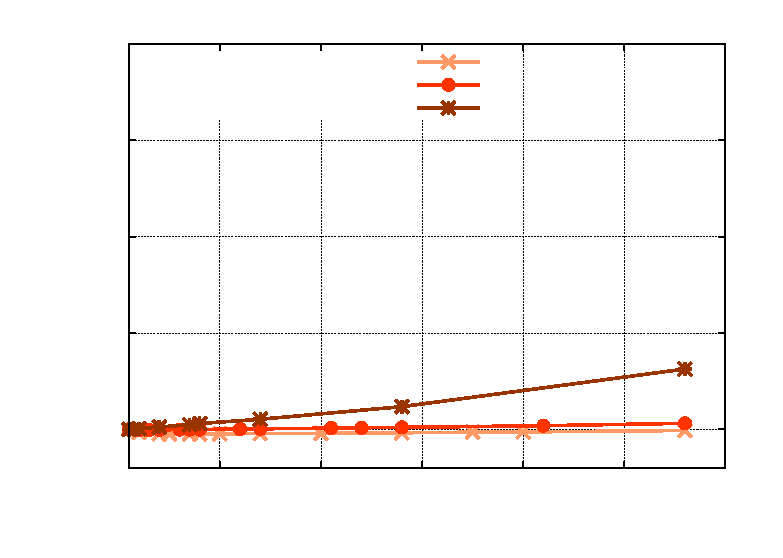
\includegraphics{plot-rowCalcT_nogatherFloat_11_500_4000_all_slide}}%
    \gplfronttext
  \end{picture}%
\endgroup
}
  \end{columns} 
\end{frame}

\end{document}

